\chapter{Resultater og analyse fra Case 1: Ulovlig fildeling på universitetsnettet til NTNU}
I dette kapittelet fremlegger vi våre resultater i alle fasene i case 1.

\section{Problemforståelse}
I denne fasen vil vi forsikre oss om at problemet er forstått i dypere detalj. Verktøyene som brukes her skal gi en bedre forståelse av omfanget og de ulike aspektene ved et problem.

\subsection{Flytdiagram}
Flytdiagrammet under viser det vi anser som et normalt hendelsesforløp til hvordan man laster ned materiale på universitetsnettverket.

\begin{figure}[H]
    \centering
    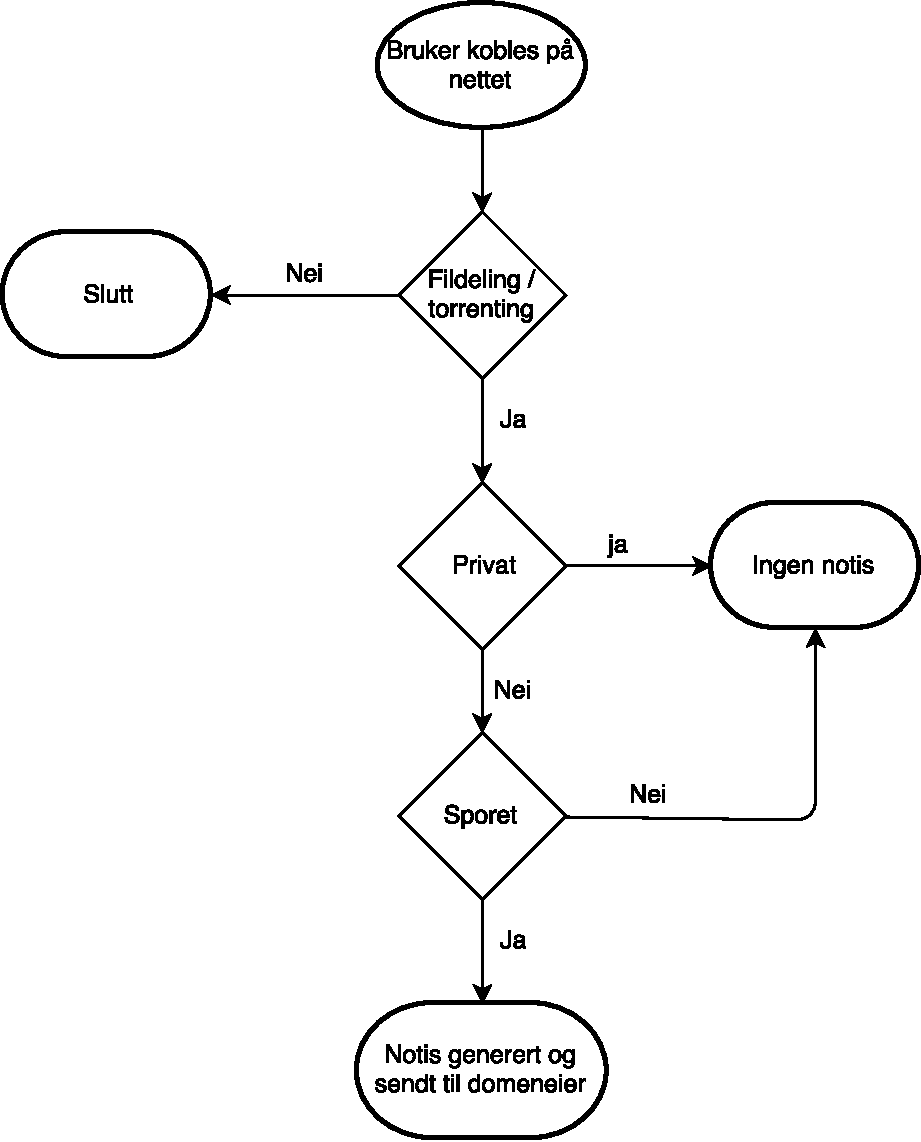
\includegraphics[scale=0.5]{case_1/bilder/Flowchart.pdf}
    \label{fig:Flytdiagram}
    \caption[Flytdiagram for fildeling]{Flytdiagram for fildeling}
\end{figure}

Først kobles en bruker seg til skolenettet, enten gjennom VPN, direkte fra campus eller studenthybler. Deretter velger brukeren enten å bruke nettet vanlig eller starter å laste ned filer, hvis brukereren bruker det vanlig bryr vi oss ikke om disse. Når vedkommende som har bestemt seg for å laste ned skal laste ned har han muligheten til å gjøre dette gjennom en privat nedlastingsside. Det neste som kan skje med de som bruker offentlige tjenester er at de torrentene de laster ned blir sporet, og da får domeneeier et notis om ulovlig nedlasting.

\subsection{Kritiske hendelser}
For å gå dypere i detalj har vi undersøkt kritiske hendelser som inngår i problemstillingen. 

Tilnærmingen fokuserte på hva studenter laster ned når de bedriver ulovlig fildeling. Derfor ble det stilt spørsmål til studenter ved Sit Bolig. På forhånd hadde vi en hypotese om at det var filmer og serier som ble lastet ned hyppigst.

Spørsmål stilt til intervjuobjekter:
\begin{itemize}
    \item Bor du, eller har du bodd i Sit-Bolig i løpet av studiet? (Hvis nei, avslutt intervju)
    \item Bruker du, eller har du brukt Torrents til å laste ned opphavsrettsbeskyttet materiale mens du bodde i Sit-bolig? Hvis ja, hvilke av følgende kategorier laster du ned fra? (Viser kategoriene)
\end{itemize}

\noindent Dette er resultatet fra spørringene: \\
\indent Antall spurt: 13 \\
\indent Antall som aldri laster ned: 4
\begin{table} [H]
    \caption[Frekvensen av ulike kategorier av nedlasting]{Oversikt over kvantiteten av kritiske hendelser ved torrenting av opphavsrettsbeskyttet materiale}
    \begin{tabular}{ | m{18em} | m{18em} | }
        \hline
            \cellcolor{yellow} Fildelingskategori & \cellcolor{yellow} Frekvens \\
        \hline
            Filmer og serier & 8  \\
        \hline
            Spill & 3 \\
        \hline
            Skolebøker & 2 \\
        \hline
            Musikk & 2 \\
        \hline
            Programvare og bøker utenom skolebruk & 1 \\
        \hline
            Programvare til skolebruk & 0 \\
        \hline
            Annet & 0 \\
        \hline
    \end{tabular}
    \label{kritisk_tabell_1}
\end{table}

Merk: Hver person kan svare at de laster ned fra flere kategorier.

\noindent Vi kan se at det er filmer og serier som er den med størst frekvens i undersøkelsen, noe som bekreftet vår hypotese. Dette funnet vil tilsi at vi kan fokusere mye mer på filmer og serier senere i prosessen siden vi vet dette er en stor del av problemet. 

\section{Idémyldring}
Denne seksjonen presenterer resultater og konklusjoner fra idémyldringsfasen. 
Problemstillingen i idémyldringen ble definert som ``Hvorfor folk torrenter på universitetsnettet''. Etter idémyldringen var ferdig ble det gjort en vurdering av resultatene og de ble kategorisert i henhold til likhetstrekk, under en fellesnevner som for eksempel Økonomi. Resultater og gruppering er som vist i figur \ref{fig:case1-idemyldring} under.  

\begin{figure}[H]
    \centering    
    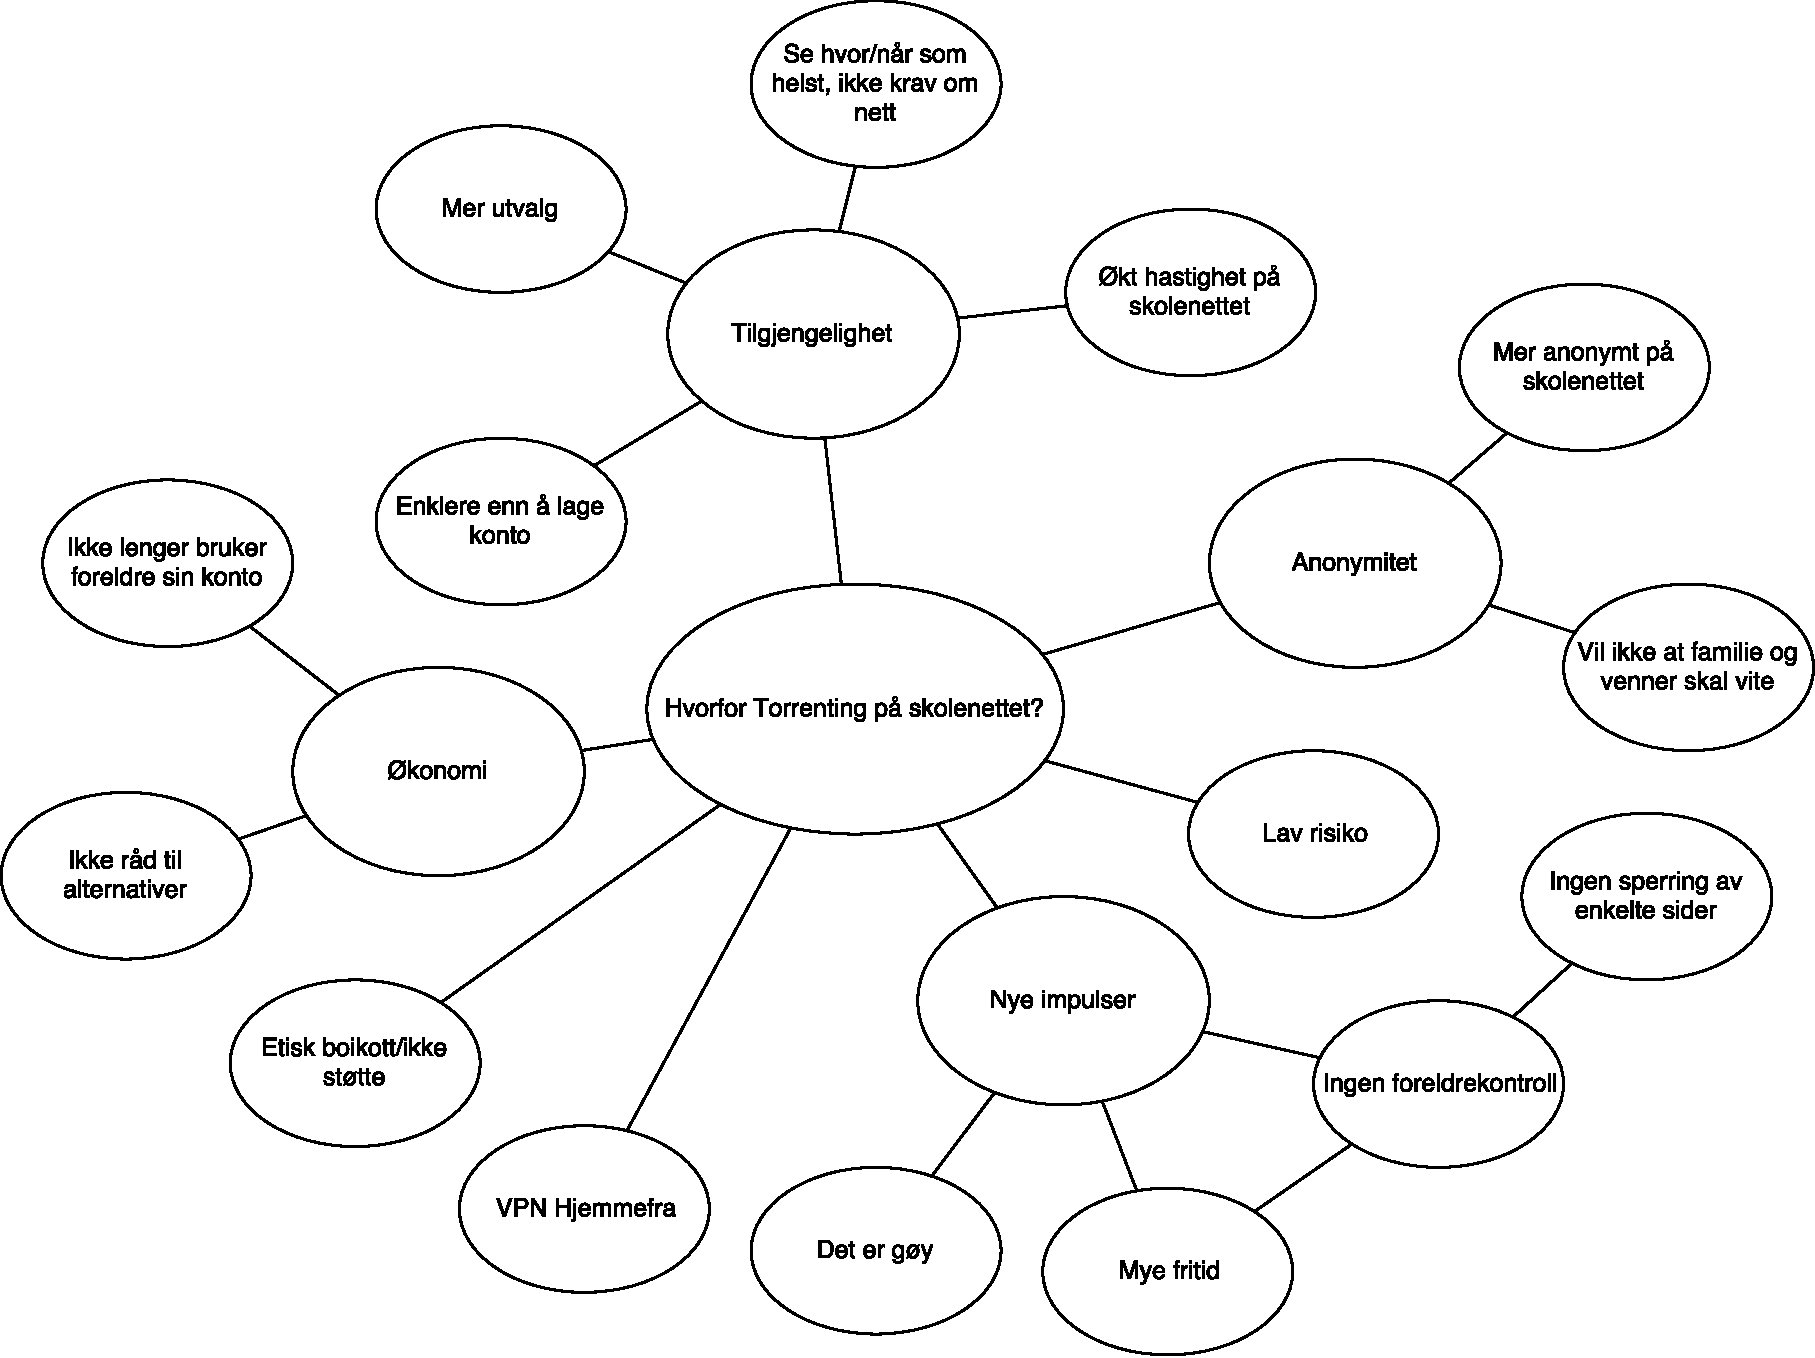
\includegraphics[scale=0.45]{case_1/bilder/idemyldring}
    \caption[Idémyldring av fildeling]{Resultater og gruppering av idémyldringen}
    \label{fig:case1-idemyldring}
\end{figure}

Resultatene er gruppert inn i fire hovedkategorier: Økonomi (som går på kjøpekraften til den enkelte person), Tilgjengelighet (hvor god tilgang en har på tjenester), Anonymitet (foreldre kunne blant annet overvåke før, samt at de føler seg tryggere når det er flere på samme nett) og nye impulser (mer frihet og fritid, og påvirkning av nedlastningskulturen).

Merk at noen årsaker kunne ikke plasseres i én kategori og er derfor direkte knyttet til problemstillingen.


\section{Datainnsamling}
Hypotesen vi går inn i undersøkelsen med er at folk laster ned opphavsrettsbeskyttet materiale fordi det er lett tilgjengelig, tilknyttet liten til ingen kostnad og ikke minst fordi det er svært lav risiko for represalier. 

Den ferdige spørreundersøkelsen finnes i vedlegg \ref{undersokelse}. 

Undersøkelsen ble begrenset til Gjøvik og endte med 97 svar totalt. Dette er 18.6\% av de 522 beboerne i Sit bolig. Av disse var det 34 som svarte at de hadde lastet ned opphavsrettsbeskyttet materiale i hybelen, det er 35\% av de spurte. 

For å øke besvarelsene ble det laget en plakat som ble lagt i postkasser og hengt opp på diverse tavler. Denne plakaten finnes i vedlegg \ref{plakat}.

Det ble også laget en engelsk versjon for de internasjonale studentene. 

\section{Dataanalyse}
I denne fasen analyseres dataene som er samlet inn, og ved hjelp av statistiske verktøy kan vi trekke konklusjoner basert på svarene. 

\subsection{Omfang}
Figur \ref{fig:case1-lasterned} under viser hvor stor andel av de 97 som ble spurt som laster ned. Rundt 35\% sier at det laster ned, som er en stor del av studentmassen. Det kan ha en påvirkning at undersøkelsen har en overvekt av studentene kommer fra informatikk- og datarelaterte studier, men det diskuterer vi nærmere senere. 

\begin{figure}[H]
    \centering
    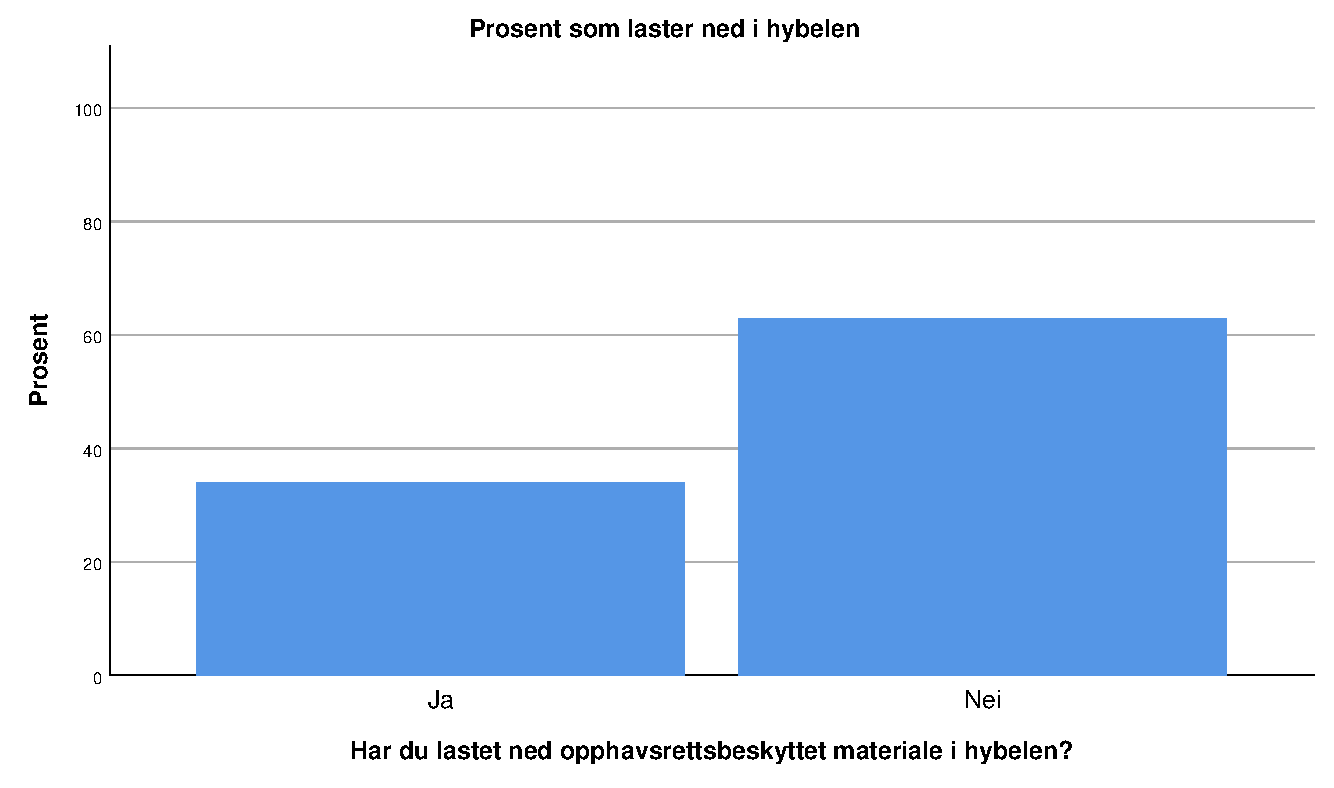
\includegraphics[scale=0.45]{case_1/bilder/lasterned.pdf}
    \caption[Hvor mange som laster ned]{Hvor mange som laster ned av de spurte}
    \label{fig:case1-lasterned}
\end{figure}

\subsection{Demografi}
I spørreundersøkelsen ble informasjon om fire forskjellige demografier samlet inn: Kjønn, fakultet, studentby og alder. Det er viktig å nevnte at det ikke ble samlet inn lik mengde svar fra alle kategoriene, så dette må vi tenke på når vi analyserer dataene. Det var for eksempel overvekt av menn som besvarte undersøkelsen. Av respondentene var det 27.8\% kvinner og 72.2\% menn. Det var også overvekt av personer som er mellom 20 og 25 år; disse tilsvarte 74.2\% av de spurte. På fakultet og studentby ønsket vi i hovedsak å få inn relativt spredte svar, men det ble overvekt av personer fra fakultet for informasjonsteknologi og elektroteknikk. I tillegg ble det også en overvekt av personer fra Kallerud studentby. Disse inkluderte henholdsvis 50.5\% og 52\% av respondentene. De komplette frekvenstabellene over demografien finnes i vedlegg \ref{frekvens}. 

\subsubsection{Kjønnsforskjeller}
Vi ønsket også å undersøke om det er noen kjønnsforskjeller i hvem som laster ned. Under ser vi forholdet mellom kjønnene.
\begin{figure}[H]
    \centering
    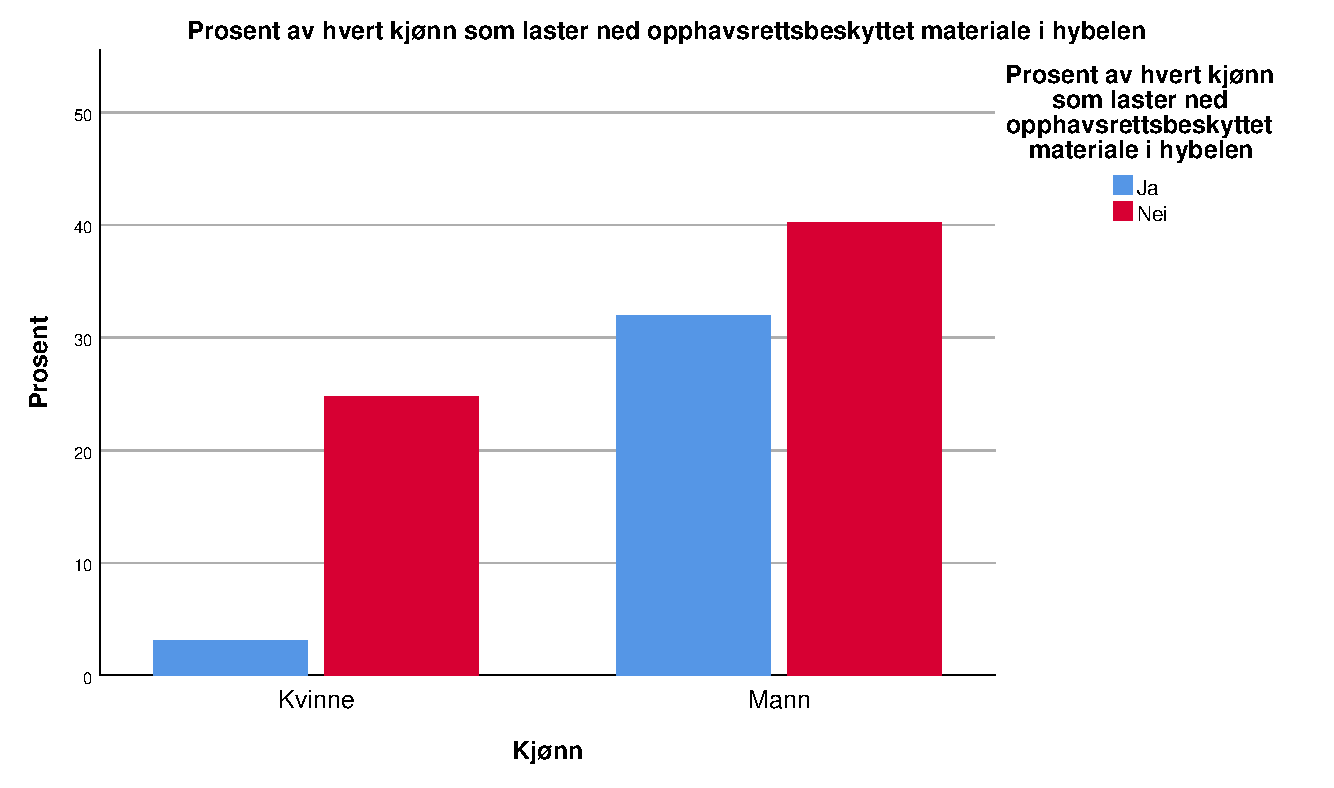
\includegraphics[scale=0.45]{case_1/bilder/kjonn_lasterned.pdf}
    \caption[Kjønn laster ned]{Hvor mange fra hvert kjønn som laster ned}
    \label{fig:case1-kjønn_lasterned}
\end{figure}
Vi kan se over at det er i hovedsak menn som laster ned ulovlig, mens kvinner har svart at de i stor grad ikke laster ned. Dette blir selvfølgelig påvirket at det er få kvinner i IT-relaterte studier, som vi har funnet ut at utgjør noe mer av nedlastingen. Det er derimot vanskelig å vite helt sikkert om det er fordi kvinner er underrepresentert i IT studier som gir utslag, eller om det er kvinner generelt sett som ikke laster ned. Der er likevel en mer signifikant forskjell mellom kjønnene enn det er mellom IT studier og andre studier som vist i figur \ref{fig:IT-lasterned}, så vi velger å tolke det som at kvinner laster ned mindre enn menn.


\subsubsection{Forskjeller mellom studentbyer}
Samtlige studentbyer har et kablet nettverk fra Uninett som er godt egnet for nedlasting, enten det er lovlig eller ulovlig nedlasting. Det er derimot noen forskjeller i hastighet på enkelte studentbyer. Kallerud har ti ganger så høy hastighet på nettet som de andre studentbyene. Derfor ønsket vi å undersøke om dette hadde noe relevans i forhold til hvor mange som laster ned ulovlig. 

\begin{figure}[H]
    \centering
    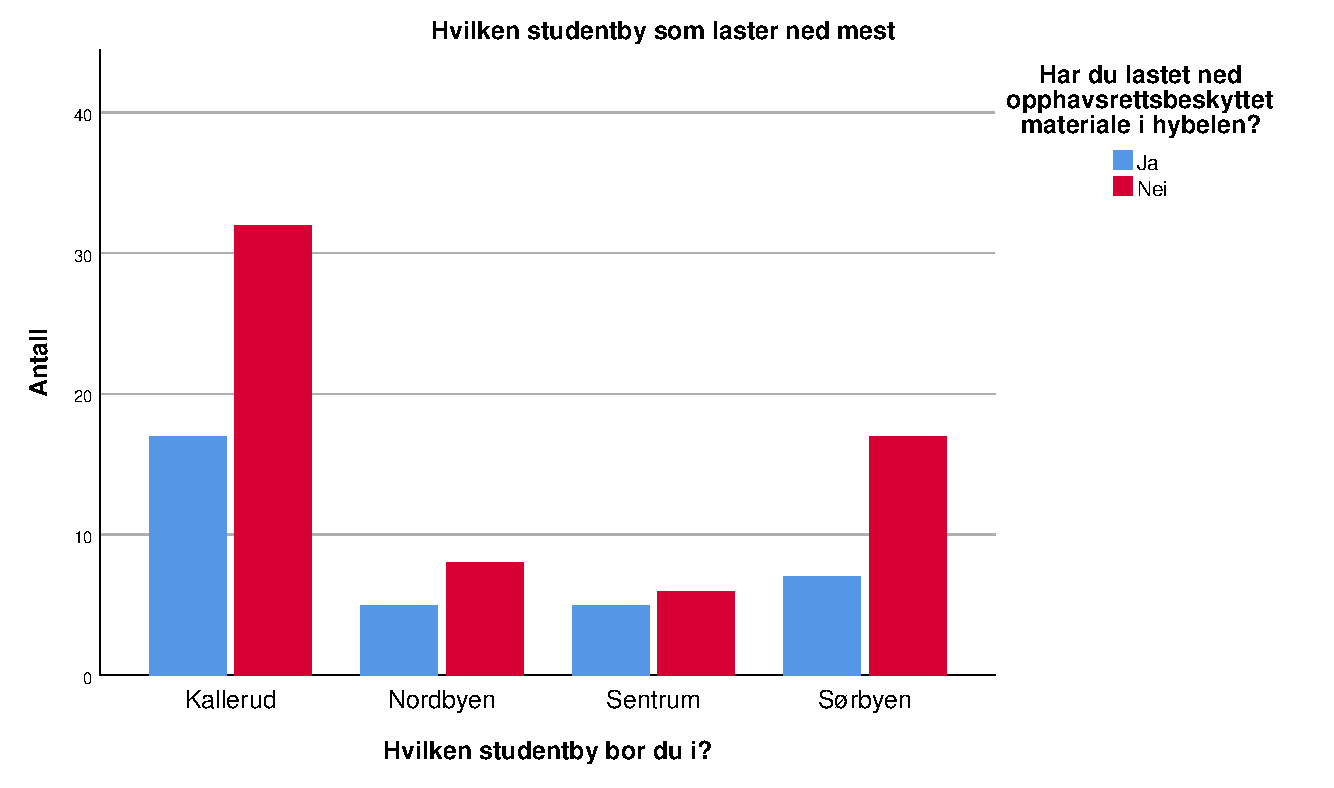
\includegraphics[scale=0.45]{case_1/bilder/studentby_lasterned.pdf}
    \caption[Studentby laster ned]{Hvor mange fra hver studentby som laster ned}
    \label{fig:case1-studentby_lasterned}
\end{figure}

På grunn av lav oppslutning på Nordbyen og Sentrum er det vanskelig å si noe sikkert på dem, mens Kallerud og Sørbyen ikke varierer så veldig fra hverandre. Når vi bruker histogrammer ser vi ingen signifikant forskjell mellom studentbyene når det kommer til nedlasting som vi kan si med sikkerhet.


\subsection{Konsekvenser ved nedlasting}
Et spørsmål som ble spurt i spørreundersøkelsen var hvor godt kjent de var med mulige konsekvenser ved ulovlig nedlasting. Det kunne være relevant å se om det var noen spesiell sammenheng mellom de som ikke kjente til konsekvensene og de som lastet ned. 

\begin{figure}[H]
    \centering
    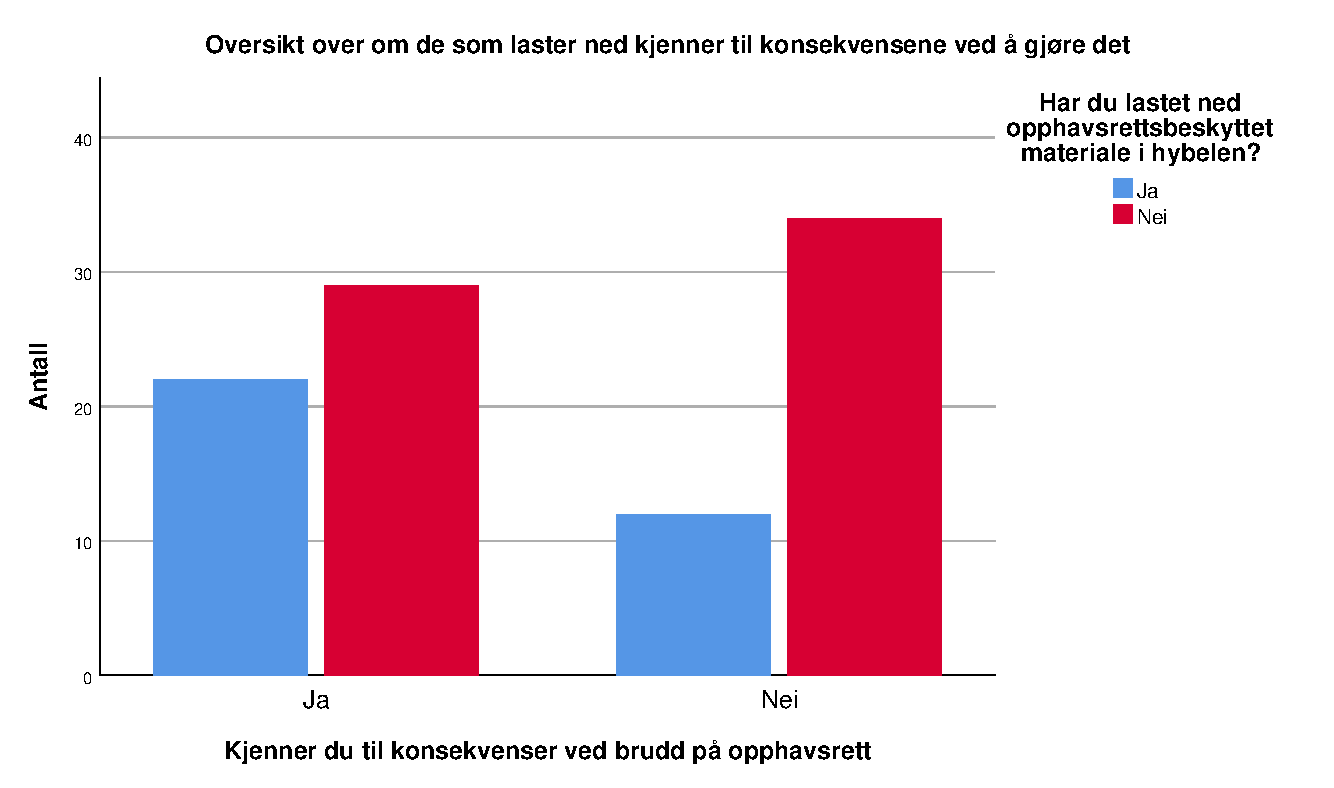
\includegraphics[scale=0.45]{case_1/bilder/konsekvens_lasterned.pdf}
    \caption[Konsekvens av å laste ned]{Hvor mange som kjenner til konsekvenser ved å laste ned}
    \label{fig:case1-konsekvens_lasterned}
\end{figure}

Det viser seg faktisk at de som laster ned har bedre kjennskap til konsekvensene enn de som ikke gjør det. Det kan kanskje ha noe å gjøre med at de er mer opptatt av problemområdet enn de som ikke laster ned. De som ikke laster ned i første omgang har kanskje ingen grunn til å sjekke konsekvensene av det. I tillegg fant vi ut at IT-studenter kjenner konsekvenser bedre enn de andre, og de har også høyere andel nedlastere. Vi prøvde å kjøre samme test på hvor godt de kjenner til IT-reglementet til NTNU \cite{ITReg} og kom til samme konklusjon som over. Dette histogrammet kan sees \hyperref[fig:reglement-lasterned]{her}. En grunn til dette kan også være at IT-studenter kjenner bedre til IT reglementet, som vist \hyperref[fig:reglement-fakultet]{her}. Og siden IT studenter er i overvekt, må dette tas i betraktning. 

En mulig teori vi ønsket å prøve ut var om mange som lastet ned ikke kjente til konsekvensene ved ulovlig nedlasting eller NTNU sitt IT-reglementet, og lastet ned på grunn av det. Dette ble altså delvis motbevist. 

\subsection{Årsaker til nedlasting}
I spørreundersøkelsen kom vi med seks påstander til hvorfor respondentene laster ned, som de besvarte på en likert-skala fra 1 til 5, der 1 er i liten grad og 5 er i stor grad. Etter å ha analysert alle seks påstandene ved hjelp av SPSS og histogrammer fant vi én påstand som hadde en graftopp der respondentene svarte positivt. De aller fleste svarte de var enige i at de lastet ned på grunn av tilgjengelighet som vist i figur \ref{fig:case1-tilgjengelighet} under.

\begin{figure}[H]
    \centering
    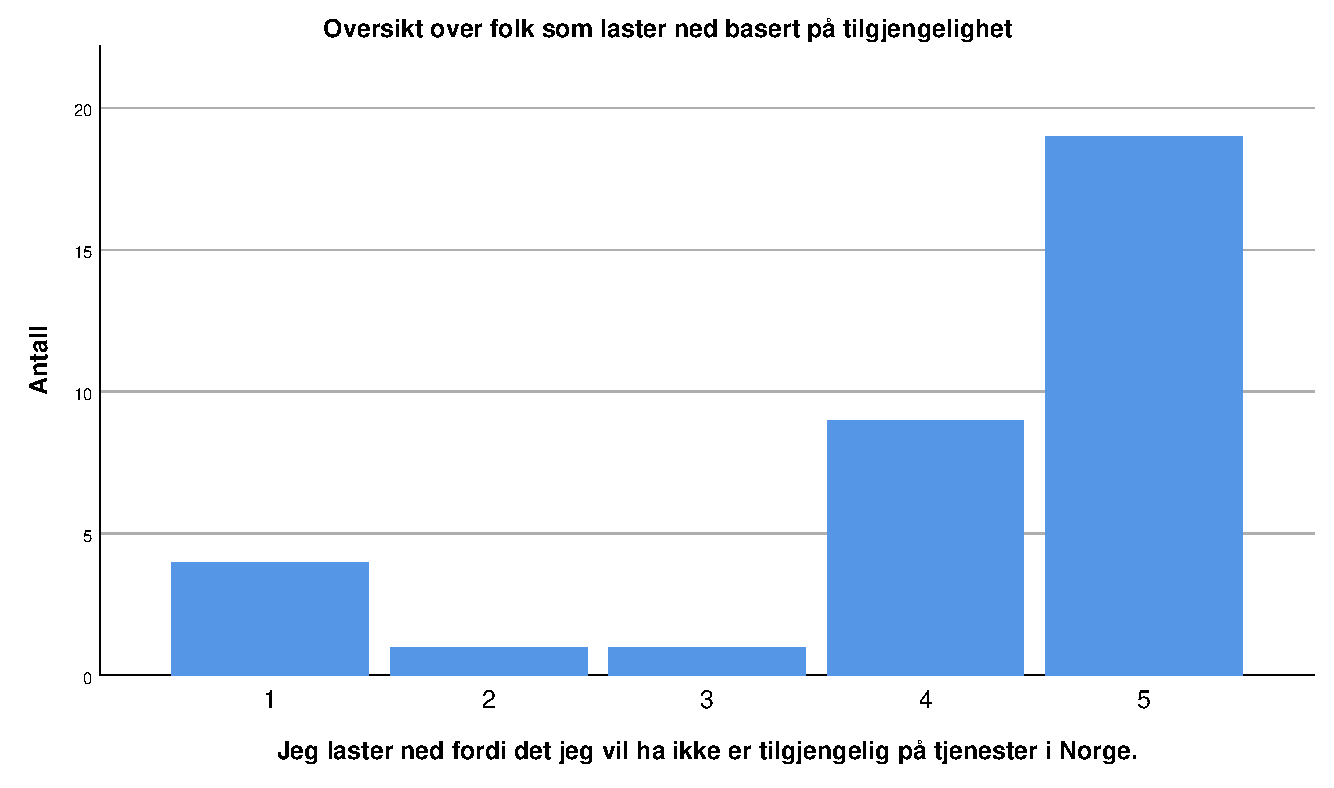
\includegraphics[scale=0.45]{case_1/bilder/tilgjengelighet.pdf}
    \caption[Laster ned pga tilgjengelighet]{Hvor mange som laster ned på grunn av tilgjengelighet av de spurte}
    \label{fig:case1-tilgjengelighet}
\end{figure}

Dette vil si at det er godt mulig at tilgjengeligheten er en årsak til om en laster ned eller ikke, og er verdt å dokumentere til videre analyse. Siden tilgjengelighet betyr så mye, var det naturlig å utforske det ytterligere. Vi fant ut at det kunne være relevant å vite om de som brydde seg om tilgjengelighet hadde tilgang på strømmetjenester, og i så fall hvor mange.

\begin{figure}[H]
    \centering
    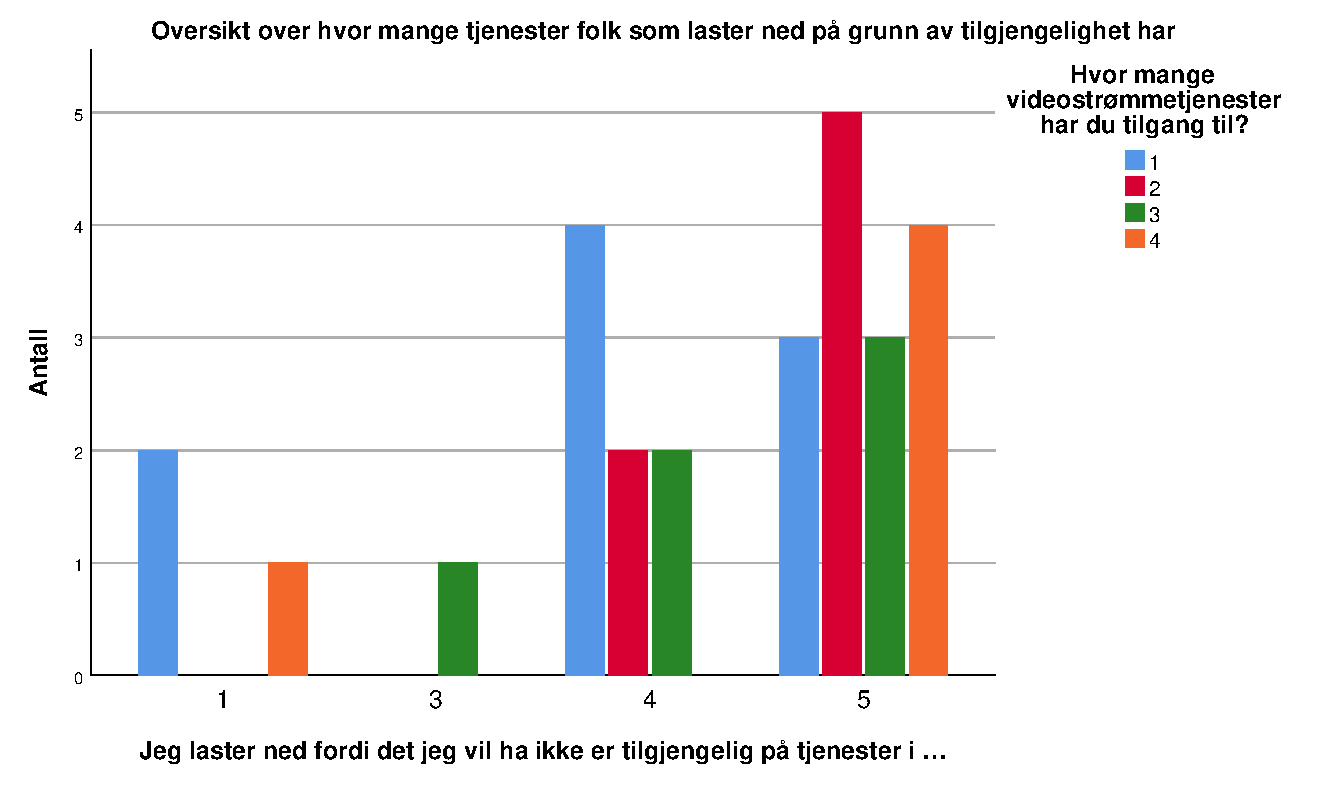
\includegraphics[scale=0.45]{case_1/bilder/tilgjengelighet_antallstromming.pdf}
    \caption[Tilgjengelighet mot antall strømmetjenester]{Korrelasjonen mellom de som laster ned på grunn av tilgjengelighet og hvor mange tjenester de har tilgang på}
    \label{fig:case1-tilgjengelighet_antallstromming}
\end{figure}

Her viser det seg at de som laster ned på grunn av tilgjengelighet også har en god del strømmetjenester. Dette sier at mange av disse er storforbrukere av film og serier, og at det ikke har så mye å si om de har tilgang til tjenestene eller ikke. Dette vil muligens utelukke en løsning i form av at NTNU tilbyr en tjeneste, siden de kommer til å laste ned uansett.

\subsection{Statistisk analyse}
I denne delen benytter vi et par statistiske verktøy for å analysere dataene. Verktøyene vi har brukt er en independent-samples t-test og en one-way ANOVA. Begge disse ble beregnet i det statistiske verktøyet SPSS. Vi regner med en signifikans på \[\alpha \le 0,05\]

\subsubsection{Independent-samples t-test}
Vi valgte å kjøre en independent-samples t-test for å undersøke om det at Kallerud har ti ganger så raskt nett har noen innvirkning på om en laster ned eller ikke. Vi delte opp Kallerud og de andre studentbyene hver for seg, og oversatte nei og ja svarene fra om du hadde lastet ned til henholdsvis 1 og 2. Under ser vi statistikken for svarene. 

\begin{figure}[H]
    \centering
    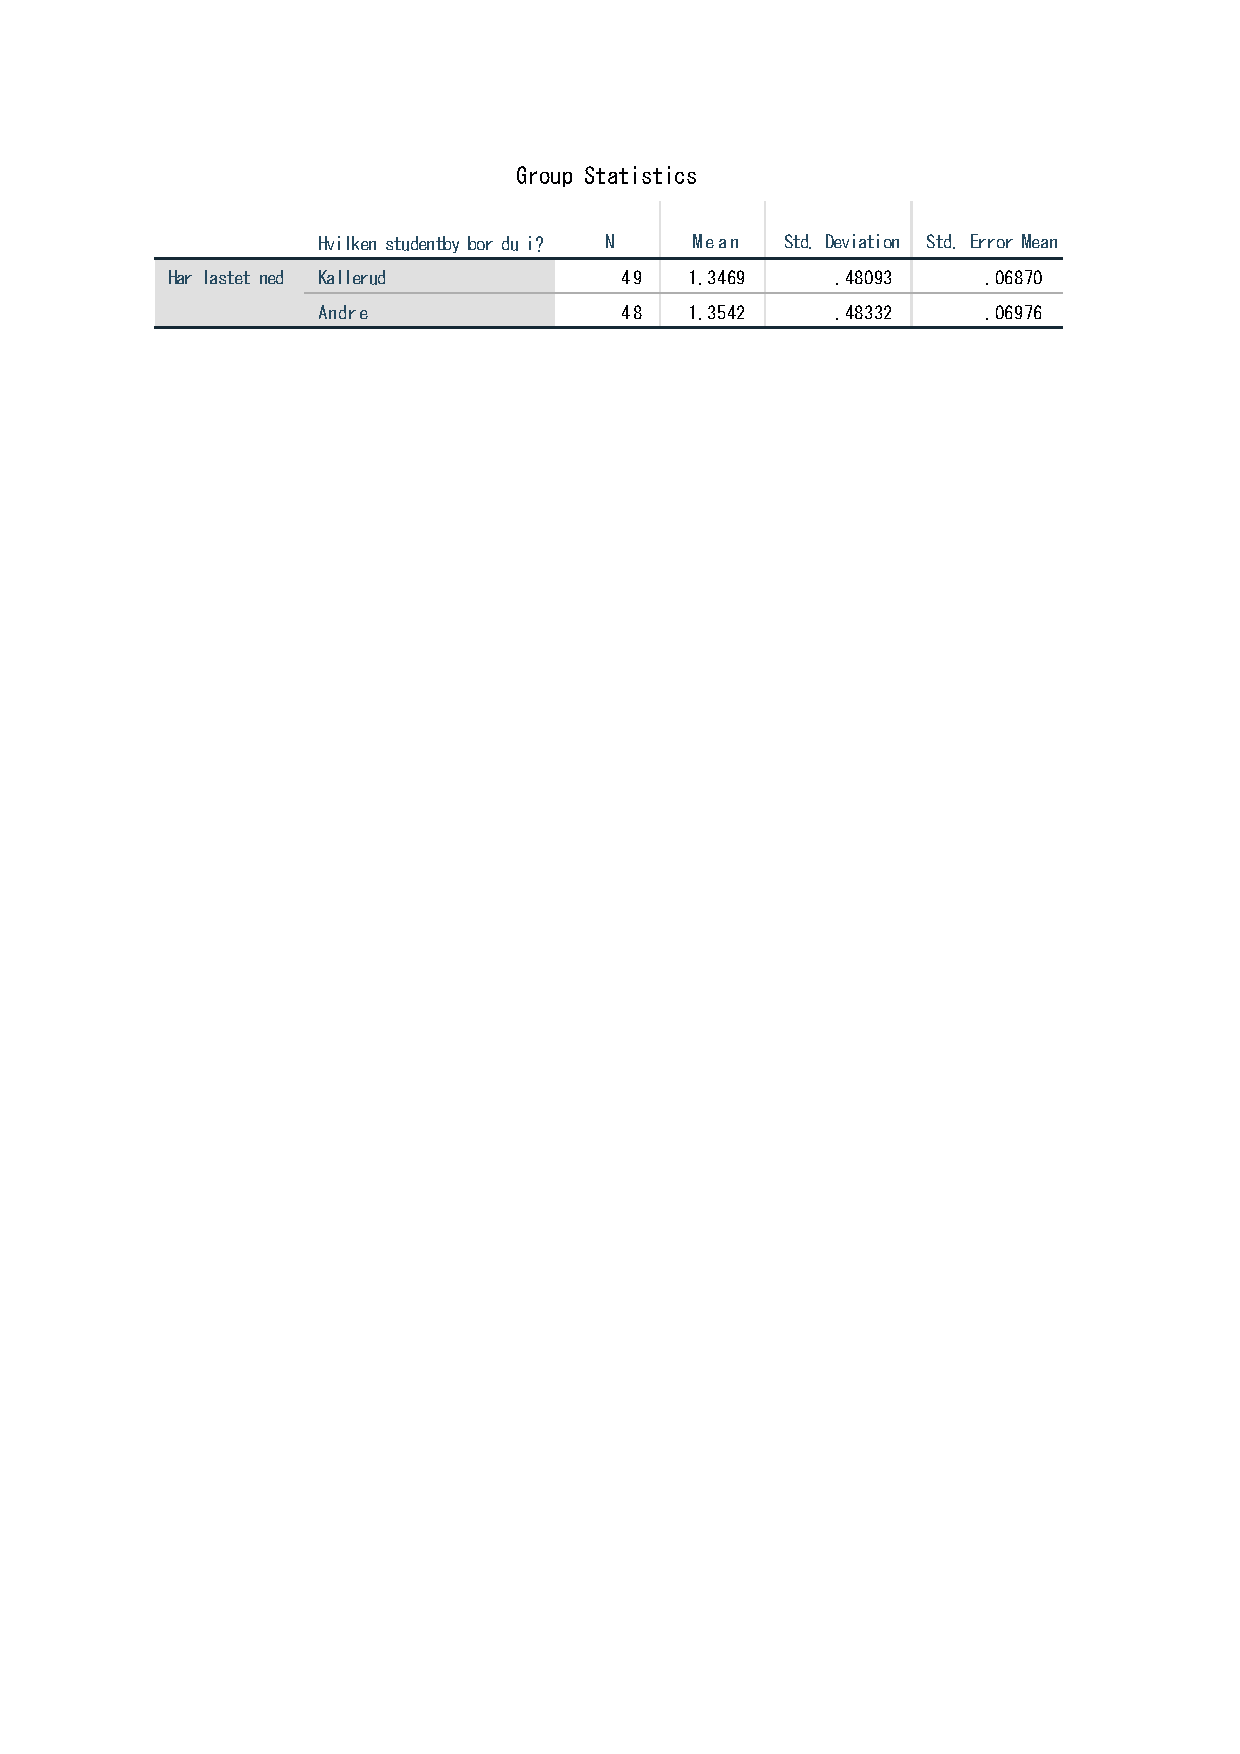
\includegraphics[scale=0.7]{case_1/bilder/studentby_lasterned_ttest_stats.pdf}
    \caption{Gruppestatistikk av studentbyer for om de laster ned eller ikke}
    \label{fig:case1-studby_lasterned_ttest_stats}
\end{figure}

Vi kan allerede her se at svarene ikke differensierer noe særlig. I testen under ser vi selfølgelig derfor at det ikke er noen signifikans.

\begin{figure}[H]
    \centering
    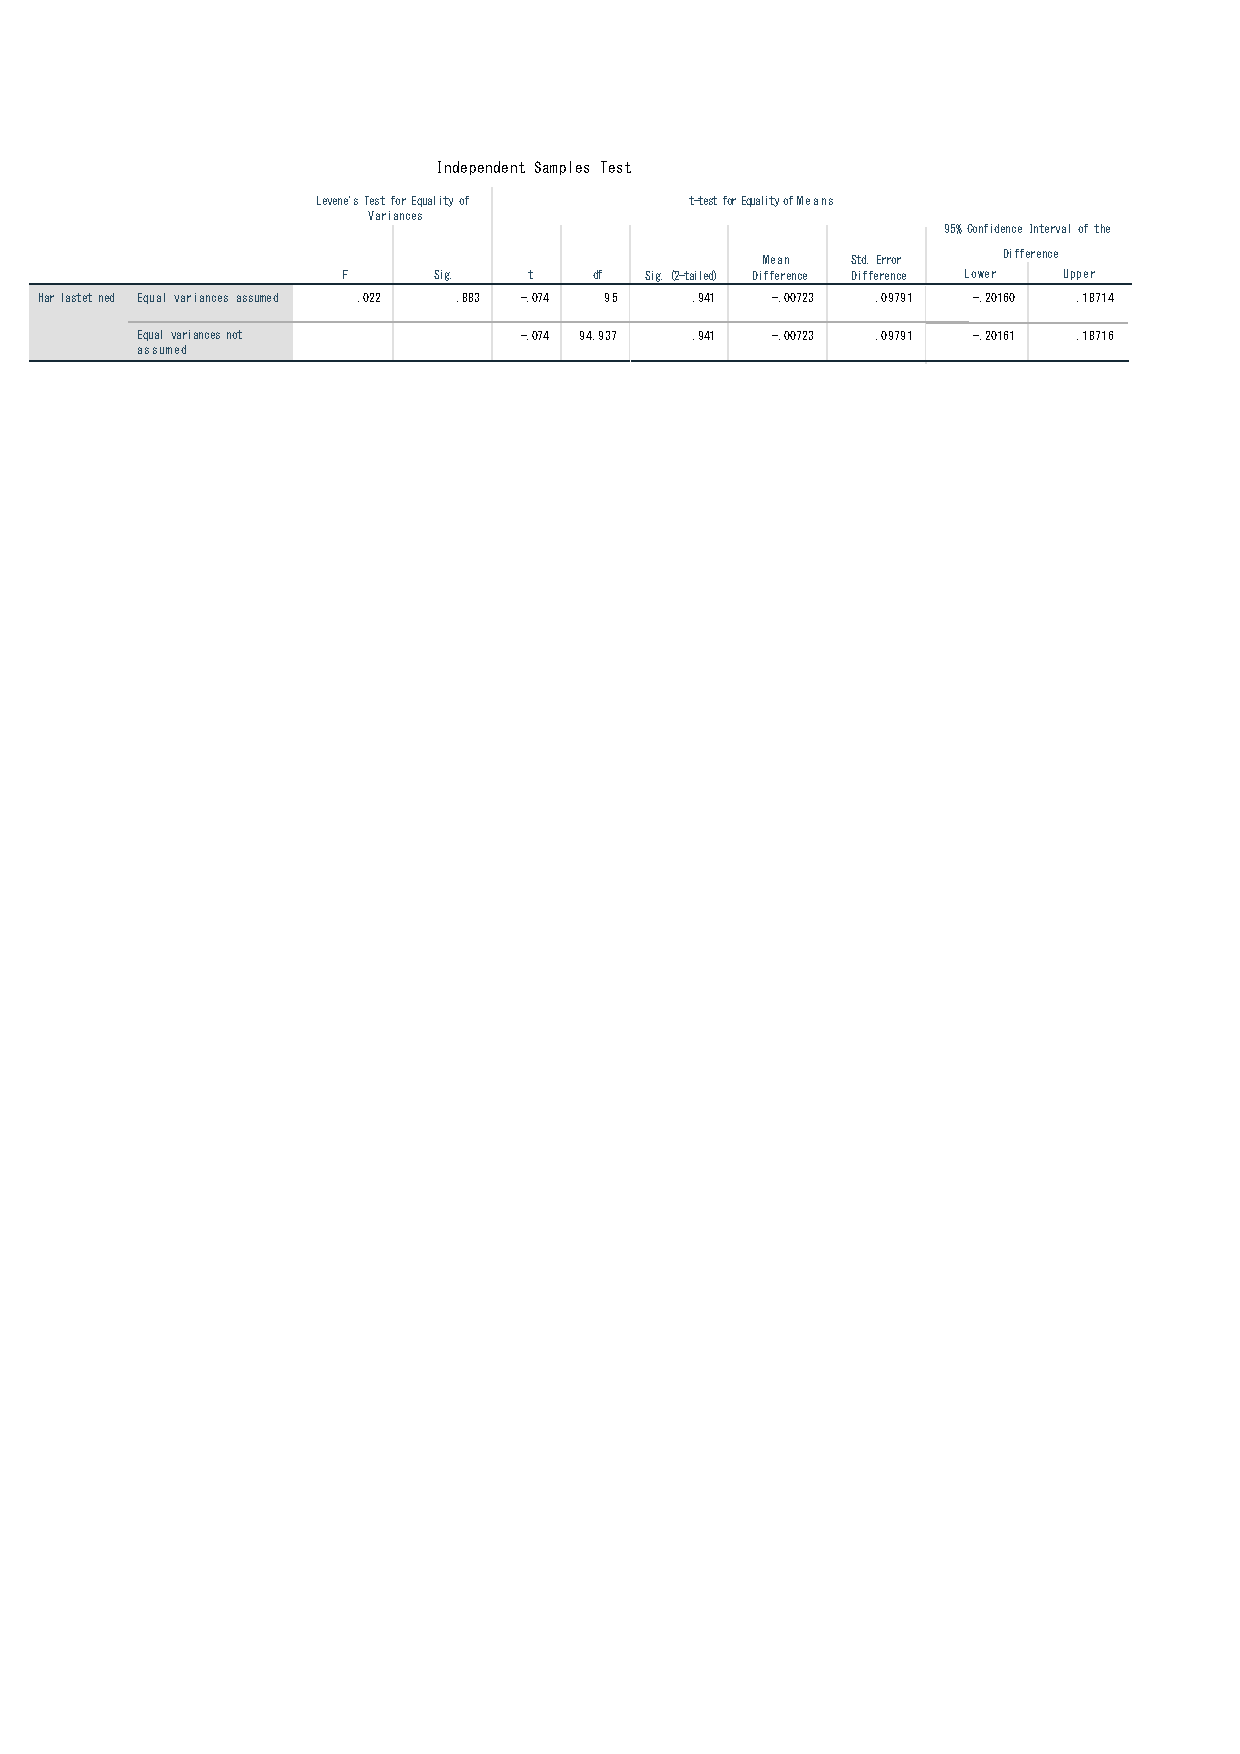
\includegraphics[scale=0.7]{case_1/bilder/studentby_lasterned_ttest.pdf}
    \caption[T-test av studentbyer mot om de laster ned eller ikke]{Independent-sample t-test av studentbyer mot om de laster ned eller ikke}
    \label{fig:case1-studby_lasterned_ttest}
\end{figure}

Dette betyr at det er ingen forskjeller på personer som bor på Kallerud og de som bor på andre studentbyer når det kommer til om de laster ned, til tross for ti ganger så rask nedlasting og opplasting. 

\subsubsection{ANOVA-analyse}
I denne analysen ser vi på forskjeller mellom IT fakultetet og de andre fakultetene i henhold til svarene som ble gitt på påstandene. Det ble i tillegg også kjørt analyser basert på kjønn og alder, men med alder var datafordelingen for lav på enkelte alternativer til å kunne si noe om det så den har uteblitt i rapporten. På kjønn brukte vi ANOVA til å se forskjeller i svar på påstandene og kjennskap til IT reglement. Bare kjennskap til IT reglement vises her siden det var det eneste med både tilstrekkelig svar fra hvert kjønn og signifikans i forskjellen.

%-----------------------------------------------ONEWAY ANOVA - fakultet MOT PÅSTAND------------------------
%-----------------------------------------------DESCRIPTIVES------------------------------------------------
\begin{figure}[H]
    \centering
    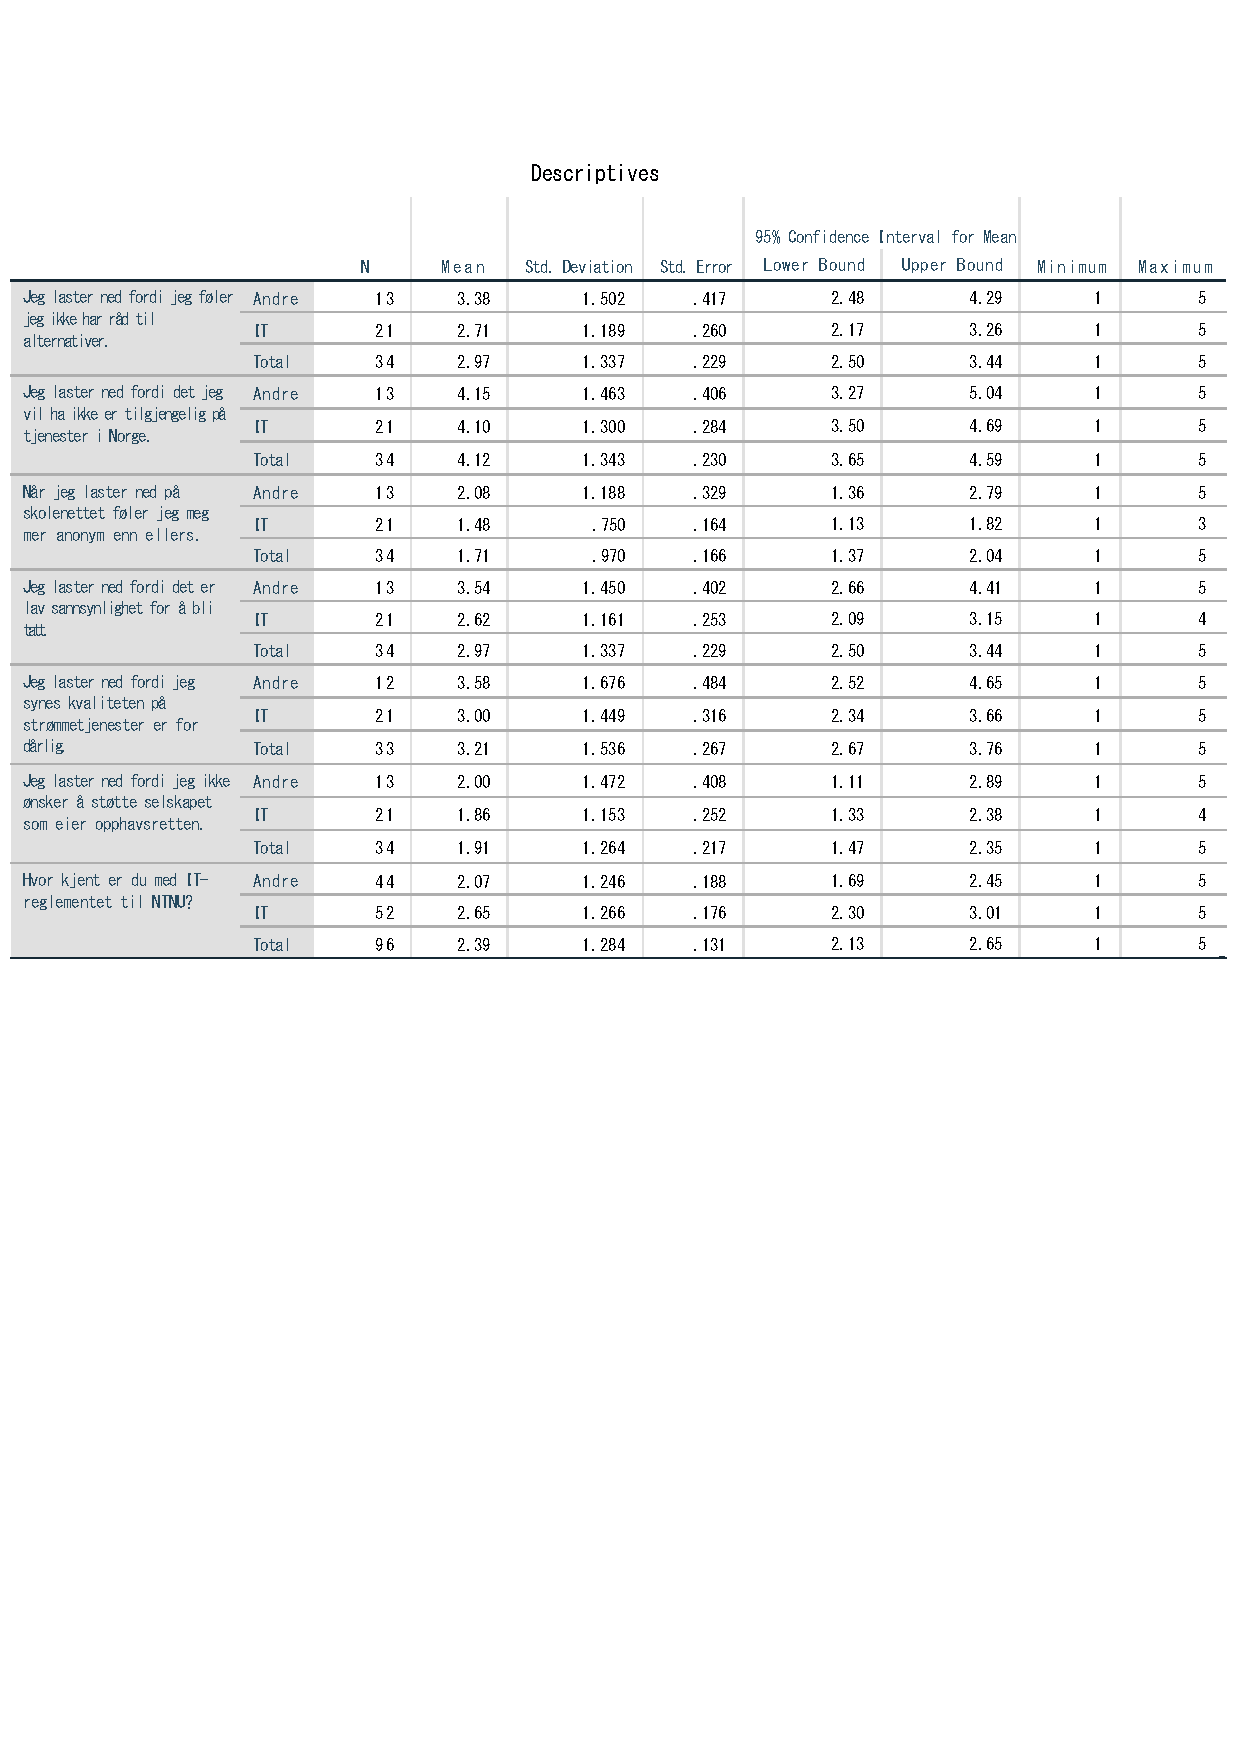
\includegraphics[scale=0.6]{case_1/bilder/fakultet_pastander_descriptive.pdf}
    \caption[Descriptives av fakultetene på påstander]{Descriptives for IT fakultetet og de andre fakultetene når det kommer til påstander}
    \label{fig:fakultet_pastander_descriptive}
\end{figure}

I tabellen over ser vi at IT studentene sier seg mer uenig i samtlige påstander, og noen mer enn andre. De svarer i tillegg at de er bedre kjent med IT reglementet. Det er spesielt påstandene om råd til alternativer, anonymitet, sannsynlighet for å bli tatt og kjennskap til IT reglementet som er mest relevant å se på. ANOVA analysen under viser om det er noe signifikans mellom svarene. 

%-----------------------------------------------ANOVA-------------------------------------------------------
\begin{figure}[H]
    \centering
    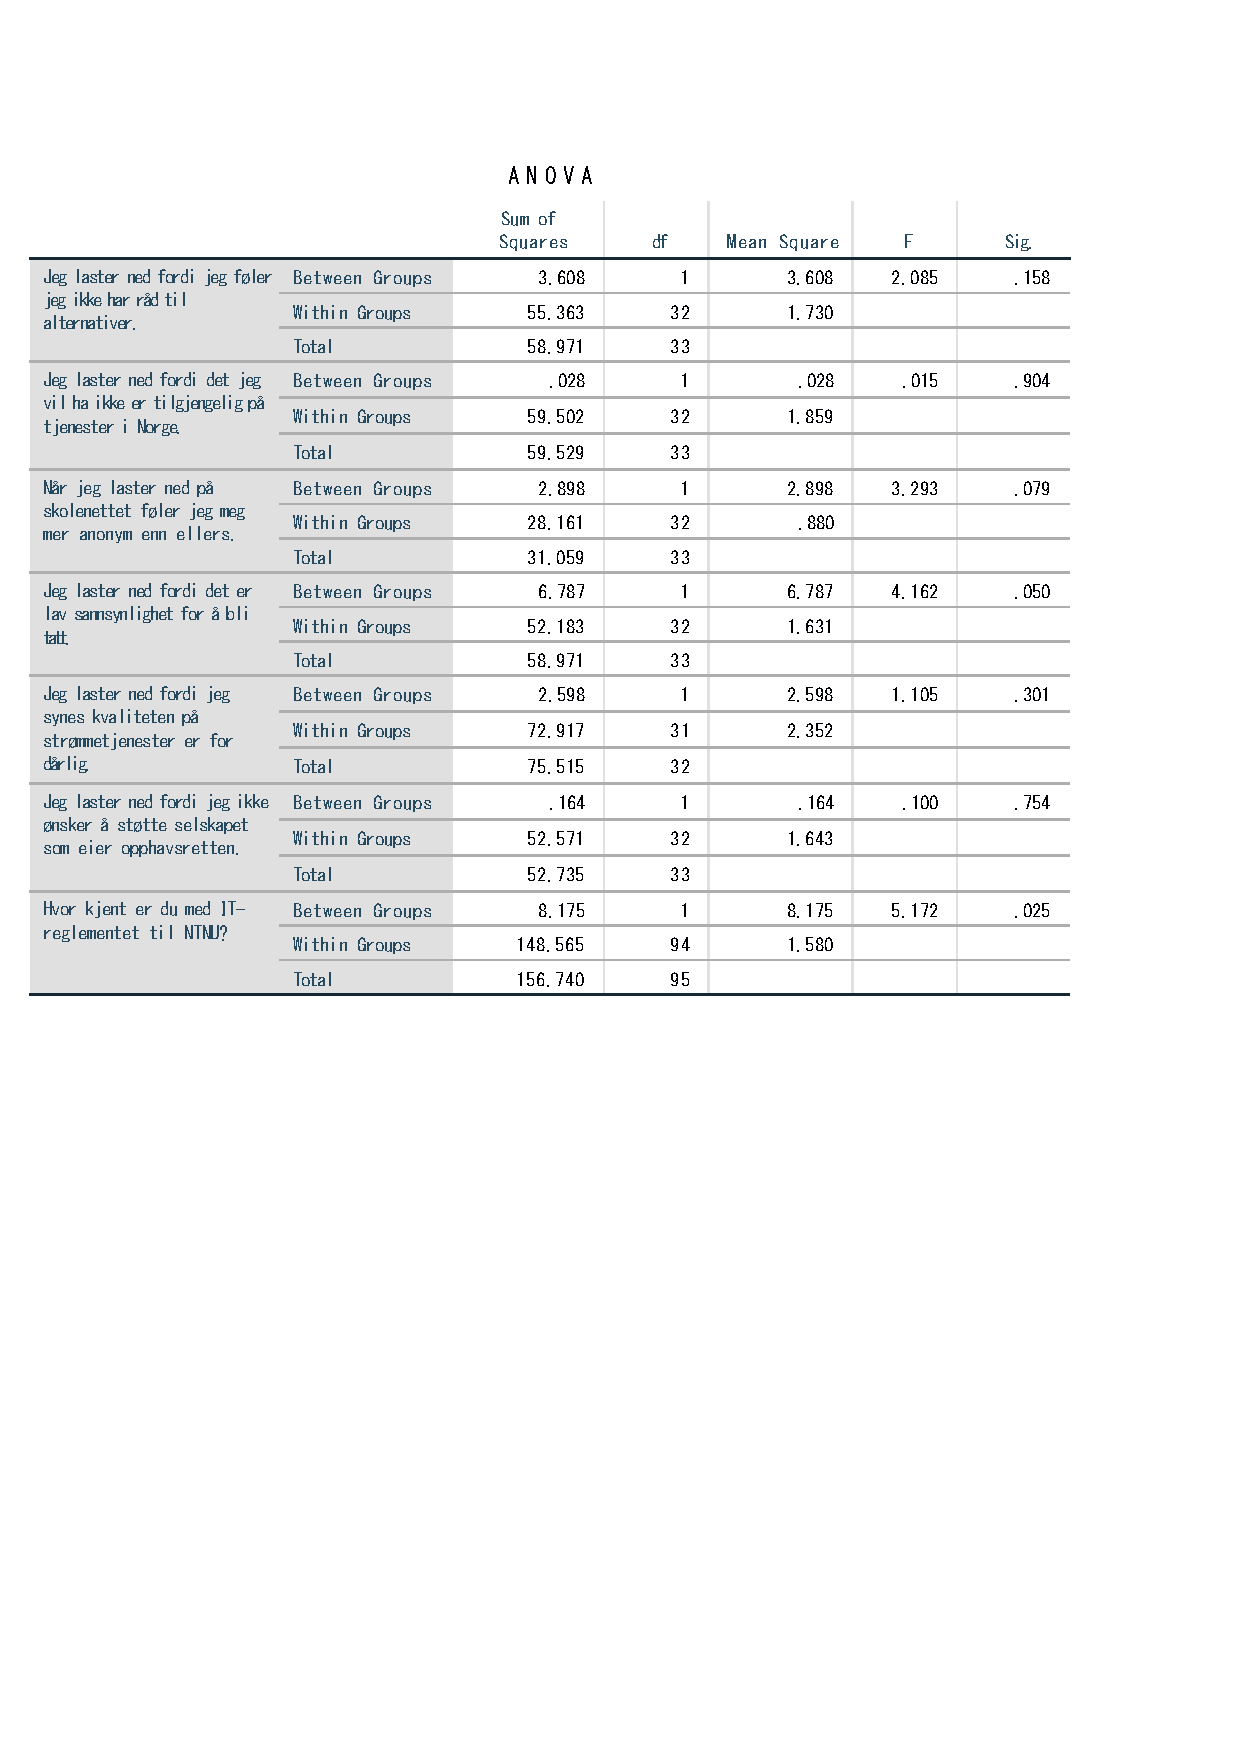
\includegraphics[scale=0.7]{case_1/bilder/fakultet_pastander_anova.pdf}
    \caption[Forskjellen mellom fakultetene på påstander]{Forskjellen mellom IT fakultetet og de andre fakultetene når det kommer til påstander}
    \label{fig:fakultet_pastander_anova}
\end{figure}

Det viser seg å være signifikant forskjell på IT og de andre fakultetene når det kommer til lav sannsynlighet for å bli tatt og kjennskap til IT reglement. Respondenter fra IT fakultetet er mer uenig i at de laster ned på grunn av lav sannsynlighet for å bli tatt \((\alpha = 0,050)\), og de kjenner også IT reglementet bedre \((\alpha = 0,025)\). 

%-----------------------------------------------DESCRIPTIVES------------------------------------------------
\begin{figure}[H]
    \centering
    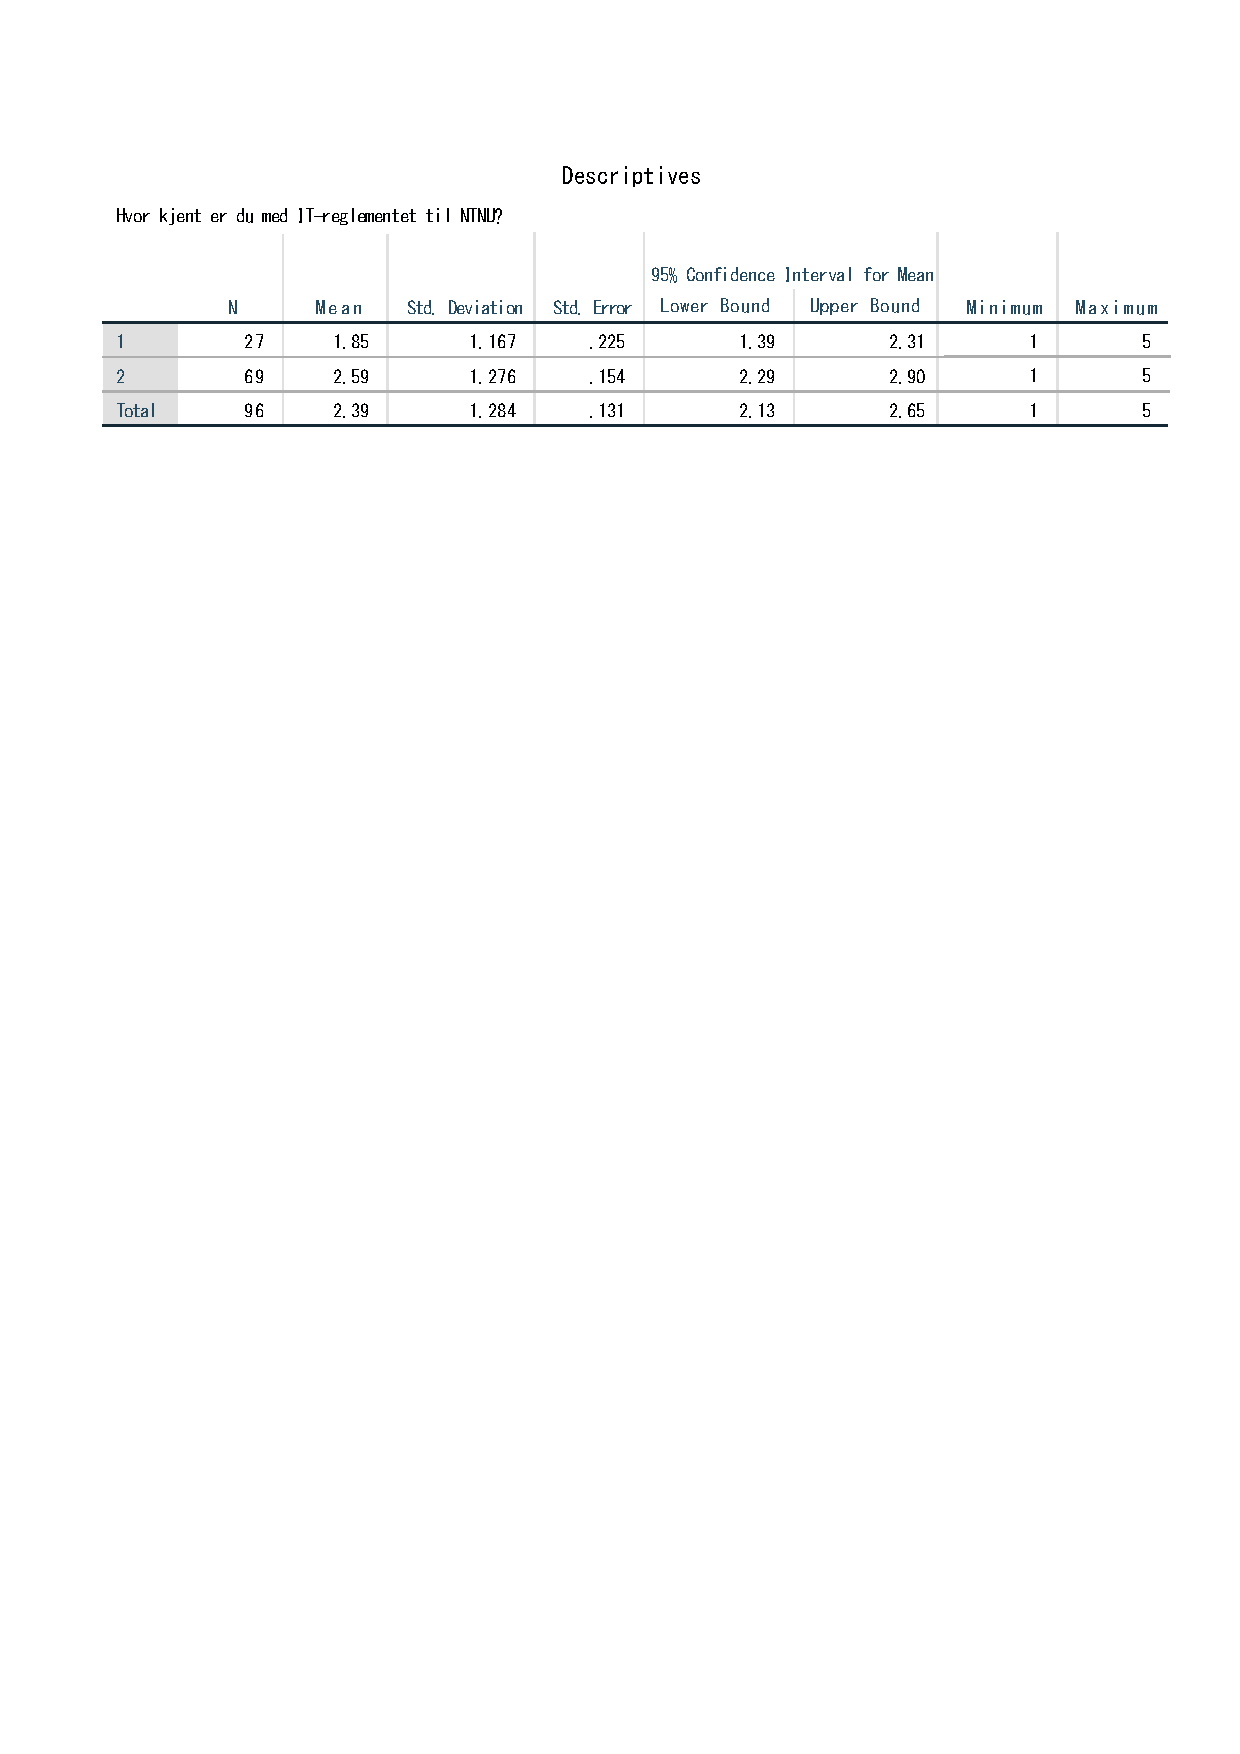
\includegraphics[scale=0.6]{case_1/bilder/kjonn_kjent_descriptive.pdf}
    \caption[Descriptives av kjønn på kjennskap til IT reglement]{Descriptives for kjønn når det kommer til kjennskap til IT reglement}
    \label{fig:fakultet_pastander_descriptive}
\end{figure}

Kvinner er 1 og menn er 2 i disse tabellene. Vi ser fra tabellen over at kvinner svarer at de kjenner til IT-reglementet noe dårligere enn menn. 
%-----------------------------------------------ANOVA-------------------------------------------------------
\begin{figure}[H]
    \centering
    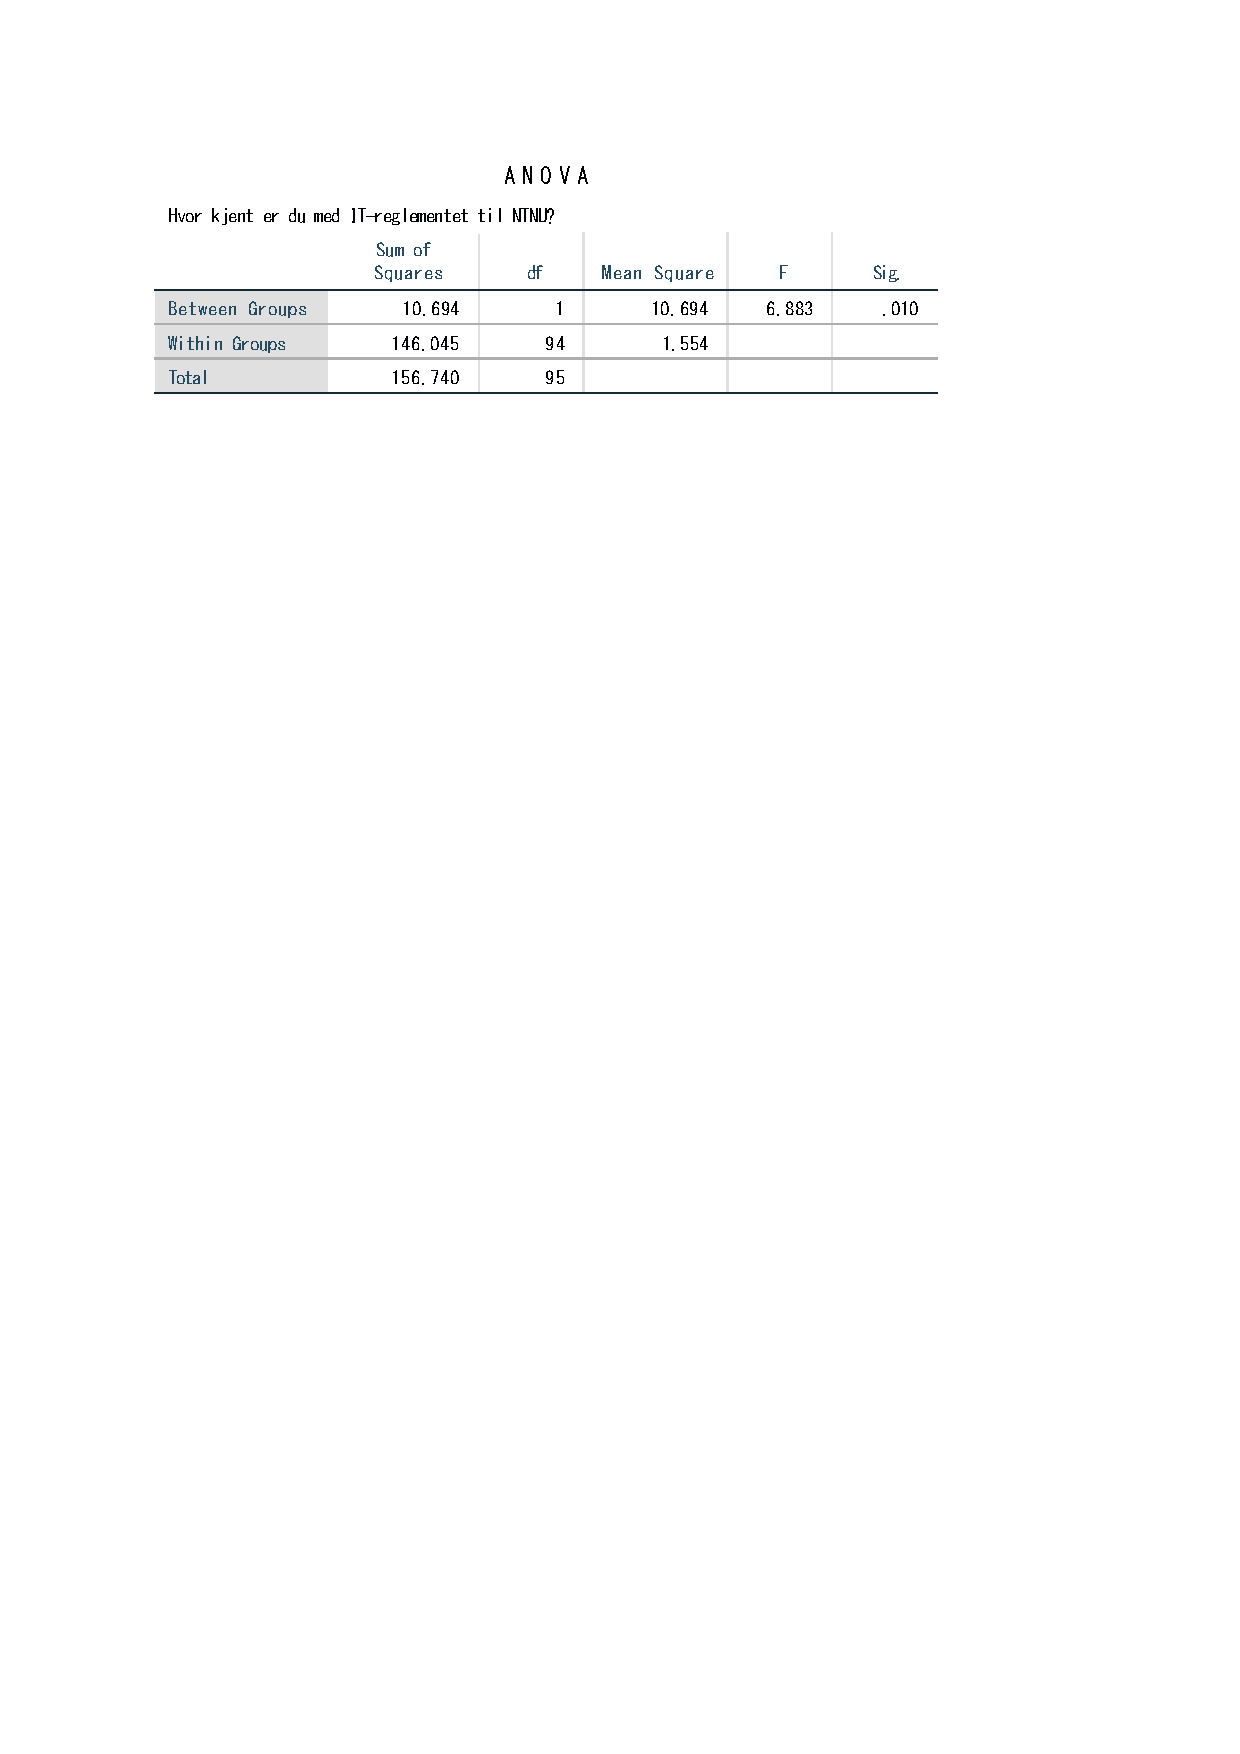
\includegraphics[scale=0.7]{case_1/bilder/kjonn_kjent_anova.pdf}
    \caption[Forskjell mellom kjønn på kjennskap til IT reglement]{Forskjellen mellom kjønnene når det kommer til kjennskap til IT reglement}
    \label{fig:fakultet_pastander_anova}
\end{figure}

I tabellen over ser vi at menn svarer at de har generelt sett bedre kjennskap til IT-reglementet, til tross for at vi fra tidligere vet at menn er overrepresentert i de som laster ned ulovlig. Noe av det kan forklares med at IT-studenter stort sett er menn, og de kjenner reglementet bedre.

\subsection{Affinitetsdiagram}
I spørreundersøkelsen spurte vi om hva som skal til for at deltagerne vil slutte med fildeling. Svarende vi fikk ble sortert inn i 16 grupper, og organisert under fire hovedkategorier. Hvis noen av deltakere har kommet med flere forslag har hvert av forslagene fått en stemme.  

\begin{figure}[H]
    \centering
    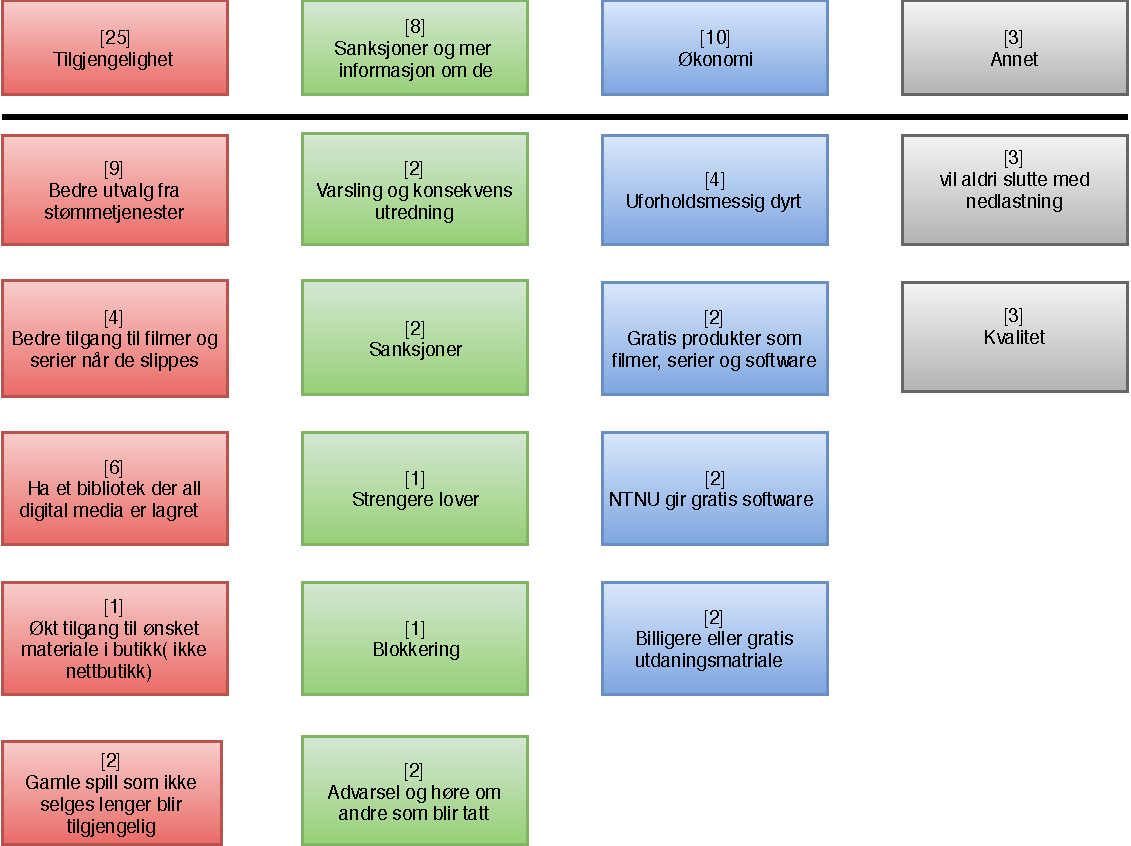
\includegraphics[scale=0.6]{case_1/bilder/stoppe_nedlastning.pdf}
    \caption[Slutte med nedlasting]{Hva skal til for at personer vil slutte med nedlasting?}
    \label{fig:case1-stoppe_nedlastning}
\end{figure}

Denne analysen gir oss ikke rotårsaken til at studenter laster ned, men kan brukes til å gi pekepinne på hva studenter mener skal til for at de vil slutte med nedlasting. Vi kan se på affinitetsdiagram at det er virker å være tre grunner til at personer laster ned. Det å gjøre materiale mer tilgjengelig virker som den beste løsningen for å stoppe personer fra å laste ned. Dette samsvarer med de tidligere funnene i figur \ref{fig:case1-tilgjengelighet}. Problemet med tilgjengelighet er at det er et mer global problem, basert på at en del av de tradisjonelle mediene fortsatt bruker geografiske begrensinger. Så da har vi igjen kategoriene økonomi og sanksjoner. Ser man på saksjoner så er det flere som mener at det å opplyse om konsekvenser og andre som blir tatt kan være et godt tiltak, som er tildels motstridende med figur \ref{fig:case1-konsekvens_lasterned}. På økonomi eksisterer det et flertall som mener at de har ikke har noe imot å betale for produktet så lenge de mener det er rimelig. Og et mindretall som vil ha gratis produkter. Her kan NTNU kanskje gjøre noe i form av muligens studentrabatter eller de betaler for produktet.

\section{Rotårsaksidentifisering}
Arbeidet i denne fasen går ut på å identifisere rotårsaken.

\subsection{Årsak-virkningsdiagram}
Problemet i fiskebeindiagrammet ble beskrevet som ulovlig fildeling på skolenettet. Hovedkategoriene vi ønsket å utforske har vi basert på dataanalysen i forrige fase for å finne de mest relevante. Disse var etter vår mening Økonomi, Risiko og Tilgjengelighet. Idémyldringen var i stor grad basert på data og funn fra analysen, med innslag fra den første idémyldringen og andre nye idéer som dukket opp.

\begin{figure}[H]
    \centering
    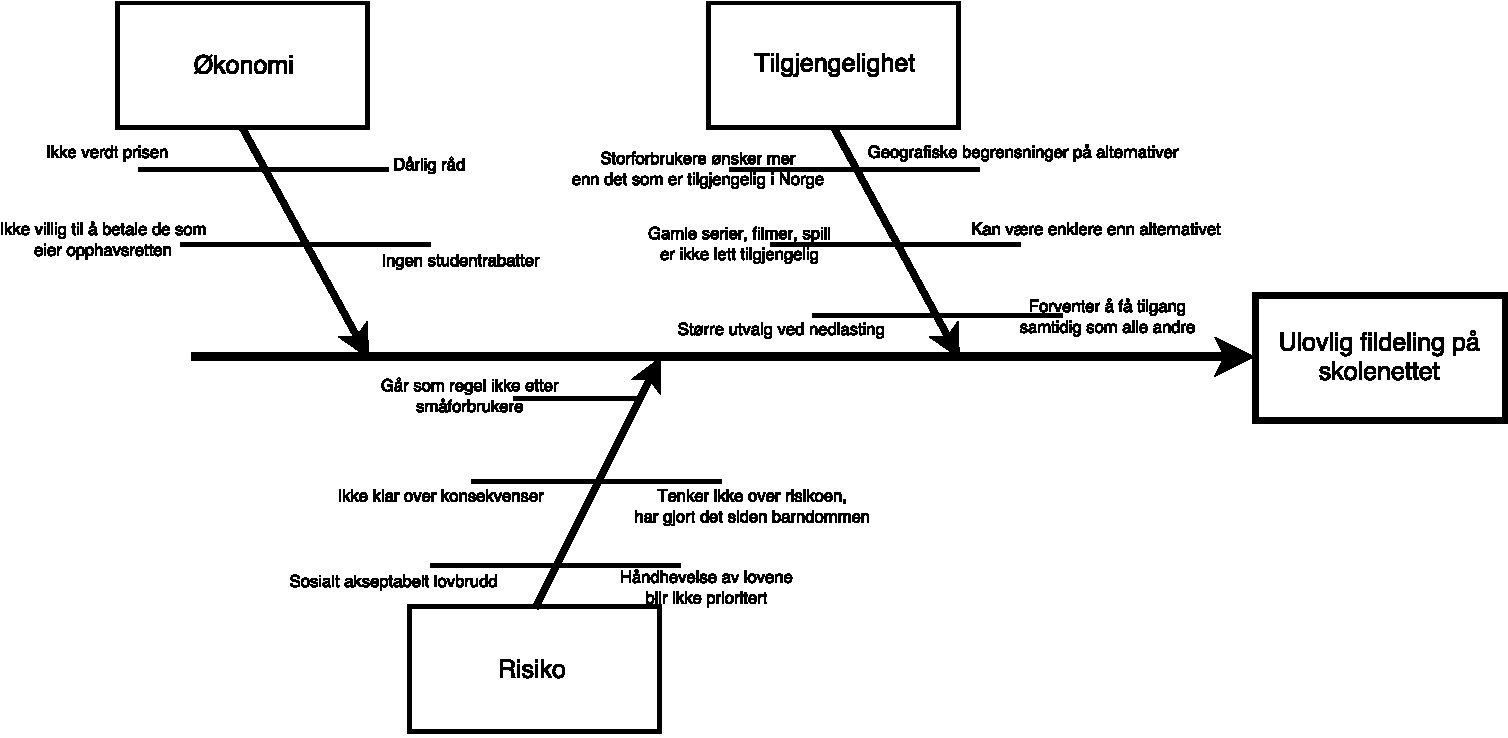
\includegraphics[scale=0.5]{case_1/bilder/fiskebein.pdf}
    \caption[Fiskebeindiagram over hovedkategorier og årsaker]{Fiskebeindiagram over hovedkategorier og årsaker}
    \label{fig:case1-fiskebein}
\end{figure}

Etter videre analyse av figuren har vi kommet frem til at rotårsaken til fildeling er en kombinasjon flere faktorer, men én skiller seg ut, nemlig tilgjengelighet. Med tilgjengelighet mener vi spesifikt at folk bedriver ulovlig fildeling fordi det er dårligere utvalg på alternative tjenester i Norge. Det finnes også noen mindre årsaker som påvirker folk til å laste ned. Blant dem er at mange føler tjenestene ikke er verdt prisen de må betale når de bare får tilgang på en begrenset mengde materiale. Den siste årsaken går på at håndheving av lovene knyttet til ulovlig fildeling ikke blir prioritert, og derfor har skapt en kultur der det er sosialt akseptabelt å laste ned. Rotårsakene er listet etter viktighet der den første er hovedårsaken:

\begin{enumerate}
    \item Dårligere utvalg på alternative tjenester i Norge
    \item Tjenestene er ikke verdt prisen
    \item Håndheving og kommunisering av lovene knyttet til ulovlig fildeling blir ikke prioritert
\end{enumerate}

\section{Rotårsakseliminering}
Arbeidet i denne fasen går ut på å finne løsninger for å eliminere rotårsaken.

\subsection{De seks tenkehattene}

Ut i fra prosessen med de seks tenkehattene kom vi fram til både gjennomførbare og ikke gjennomførbare tiltak. 
\subsubsection{Gjennomførbare tiltak}
\begin{itemize}
    \item Tilby produkter fra selskap som universitetet får flest notifikasjoner fra.
    \item Stenge torrentprotokollen for alle på nettverket.
    \item Grense på nedlastning og opplastning av data.
    \item Være strengere når det gjelder oppfølging av IT-reglementet. 
    \item Bytte ISP til studentboligene.
    \item Oppmerksomhetskampanje om konsekvenser.
    \item Avtale med kino for billige eller gratis nye filmer
\end{itemize}

\subsubsection{Ikke gjennomførbare tiltak}
\begin{itemize}
    \item Alt av materiale blir gratis og tilgjengelig på ett samlet sted
    \item Fjerne geografiske blokkeringer
\end{itemize}

Noen av disse vil ikke være gjennomførbare for NTNU så vi har valgt å ikke ta de med videre til implementering, men de er fortsatt interessante å nevne. Av de 11 forslagene er det kun 4-5 vi mener har høy sannsynlighet for å bli kvitt rotårsaken, helt eller delvis; eller flytter rotårsaken vekk fra NTNU ansvarsområde. Etter videre vurdering har vi kommet fram til de mest lovende løsningene for å fjerne rotårsaken. Disse beskrives i ytterligere detalj under.

\subsubsection{Tiltak som fjerner rotårsaken til at folk laster ned}

\begin{enumerate}
    \item Alt av materiale blir gratis og tilgjengelig på ett samlet sted
    \item Fjerne geografiske blokkeringer
    \item Tilby produkter fra selskap som skolen får mest notis fra
    \item Prøve for studenter for å få full hastigehet på nettverk
\end{enumerate}

\subsubsection{Tiltak som fjerner rotårsaken til at skolen får notifikasjon fra opphavsrettshaverne}

\begin{enumerate}
    \item Bytte ISP til studentboligene
    \item Stenge torrentprotokollen for alle på nettverket
\end{enumerate}

Rotårsaken til at folk bedriver ulovlig fildeling er ikke et problem som lett kan løses av skolen. Vi har gitt et par forslag til hva som kan fjerne rotårsaken helt, men av disse er ikke alle gjennomførbare for skolen. Vi har også foreslått et par tiltak som ikke fjerner rotårsaken og noen som fjerner rotårsaken til hvorfor folk laster ned. De tiltakene som ikke fjerner rotårsaken vil flytte rotårsaken bort fra NTNU sitt ansvarsområde.

\subsection{Systematisk Innovativ Tenkning (SIT)}
Alle komponenter som eksisterer i problemets naturlige omgivelser listes under:

\begin{itemize}
    \item Lite kunnskap om konsekvenser
    \item Raskt internett
    \item Alt er tilgjengelig samtidig overalt
    \item Økonomi
  %  \item Kjedsomhet - laste ned serier/spill for å ha noe å gjøre
\end{itemize}

På hver komponent blir de fem hovedprinsippene fra SIT brukt til å myldre frem idéer på ulike tiltak som kan fjerne rotårsakene eller bedre problemet.

\paragraph{Lite kunnskap om konsekvenser}
\begin{itemize}
    \item \textbf{Attributtavhengighet} Løfte opp kunnskapen om konsekvenser og lover.
    \item \textbf{Komponentkontroll} Ha en test for å se at folk forstår IT-reglementet og mulig kursing.
    \item \textbf{Erstatning} Ikke gjennomførbart
    \item \textbf{Forkastning} Ikke gjennomførbart
    \item \textbf{Oppdeling} Ikke gjennomførbart
\end{itemize}

\paragraph{Raskt internett som skolen eier}
\begin{itemize}
    \item \textbf{Attributtavhengighet} Sperre torrenting protokollen.
    \item \textbf{Komponentkontroll} Ikke gjennomførbart.
    \item \textbf{Erstatning} Ha tregere internett, slik at folk ikke laster ned hjemme.
    \item \textbf{Forkastning} Fjerne internett fra Sit boligene/bytte ISP.
    \item \textbf{Oppdeling} Ikke gjennomførbart
\end{itemize}

\paragraph{Tilgjengelighet}
\begin{itemize}
    \item \textbf{Attributtavhengighet} Få rettighetshaverne til å samle alt innhold til ett sted 
    \item \textbf{Komponentkontroll} Ikke gjennomførbart.
    \item \textbf{Erstatning} Tilby gratis filmer/serier og spill.
    \item \textbf{Forkastning} Ikke gjennomførbart
    \item \textbf{Oppdeling} Ikke gjennomførbart
\end{itemize}

\paragraph{Økonomi}
\begin{itemize}
    \item \textbf{Attributtavhengighet} Mer penger fra lånekassen. 
    \item \textbf{Komponentkontroll} Skolen tilbyr det som blir lastet ned mest
    \item \textbf{Erstatning} Skolen gjør innhold gratis
    \item \textbf{Forkastning} Ikke gjennomførbart
    \item \textbf{Oppdeling} Ikke gjennomførbart
\end{itemize}

Løsningene sorteres deretter og diskuteres ut fra hvilke som er mest relevante. 

\begin{description}
    \item[Lite kunnskap om konsekvenser] Løfte opp kunnskapen om konsekvenser og lover.  Måten vi kan gjøre dette på er å ha et kurs og dette kurset kan ha en påfølgende quiz.
    \item[Raskt internett som skolen eier] Det å sperre torrenting protokollen er nok ikke gjennomførbart fordi skolen er eneste internettleverandør. Det å bytte ISP ved studentboligene er mulig, men vil kreve videre utredning.
    \item[Tilgjengelighet] Det at alt materialet blir samlet på ett sted vil være en krevende prosess.
    \item[Økonomi] Skolen sjekker hva som blir lastet ned mest og prøver å få til en avtale med rettighetshaverne om en billig god måte å få tilbudt dette til studentene.
    %\item[Kjedsomhet] Ha en bedre informasjonskanal enn facebook for å få delt ut informasjon om de ulike aktivitetene på skolen.
\end{description}

Deretter diskuteres løsningene videre og de mest lovende ideene blir med i tiltaksplanen. Vi tror de mest lovende idéene er følgende:

\begin{description}
    \item [Kurs] Skolen tilbyr et kurs, gjerne ett nettkurs, med en tilhørende prøve for å se hvor mye folk får med seg.
    \item [Bytte ISP] Bytter Sit ISP vil ansvaret for notisene flyttes fra universitetet til den nye ISP. 
    \item [Tilby produkter] Her kan skolen se gjennom de ulike notisene de har fått, og finne ut hvilket selskap som blir lastet ned mest, for så å prøve å tilby deres filmer og serier.
    \item [Alt materialet tilgjengelig] Om alt materialet er tilgjengelig på ett sted vil dette fjerne problemet med at eneste og/eller enkleste måten å få tak i produkter er ved å laste dem ned.
\end{description}

\section{Løsningsimplementering}
Arbeidet i denne fasen går ut på å utrede en tiltaksplan og lage et forslag til hvordan dette skal implementeres.

\subsection{Tiltaksplan}
Gjennomføring av disse tiltakene vil i hovedsak administreres av universitetet og Sit.

\subsubsection{Alt av materiale blir gratis og tilgjengelig på ett sted}
Dette tiltaket vil fjerne rotårsaken helt og holdent. Alt materiale blir gratis, gitt ut på samme tid over hele verden og tilgjengelig på ett sted. Dette tiltaket har svært høy kost, men også høy nytte. Skolen må skaffe avtaler med alle produsenter og tilby det til studentene. Dette vil fjerne rotårsaken, men er urealistisk. 

\subsubsection{Tilby produkter fra selskap som universitetet får flest notiser fra}
Går ut på å finne de mest populære selskapene som universitetet får notis fra, skaffe en avtale med rettighetshaverne eller som er distributør for rettighetshaverene og gjøre dette tilgjengelig for studenter. Dette vil fjerne rotårsaken på at de laster ned fra dette selskapet. Dette har middels start kostnad som starter med å kartlegge hvilke firmaer som har høy frekvens av notiser. Kostnaden tilknyttet dette tiltaket er i hovedsak det å få til en avtale med rettighetshaverene, eller distributørene av materialet i Norge.

\subsubsection{Kurs for studenter i bruk av universitetsnettet}
Etablere et kurs for studenter om hvordan man skal bruke universitetsnettet. Nye studenter som kommer til NTNU vil ha som krav å gjennomføre kurset, som en del av signereingen av IT reglementet. Kurset kan avluttes med en test, for å se hvor mye av IT reglementet studenten har fått med seg. Denne testen kan muligens brukes i forbindelse med initiativ eller straff ettersom hvor godt studenten gjør det. Dette kurset kan bli for omfattende for hele universitetet og kan heller bare bli gitt til Sit leietakere. Dette prosjektet kan bli både tidkrevende og ha en høy kostnad, så vi foreslår for å begrense ressursbruken at dette prosjektet blir en mulig bacheloroppgave. 

\subsubsection{Sit bytter ISP}
Det å bytte ISP eller splitte studenthjemmene fra skolenettverket vil være en dyr og tidkrevende prosess, men dette kan være verdt å gjennomføre. Dette vil ikke fjerne rotårsaken til problemet, men vil flytte problemet vekk fra NTNU sitt ansvarsområde.

\subsection{Trediagram}
For å implementere tiltakene beskrevet over brukes trediagram for å strukturere og dele opp aktivitetene som må gjøres. Dette vil fungere som et enkelt utkast til en prosjektplan. 

\begin{figure}[H] 
    \centering    
    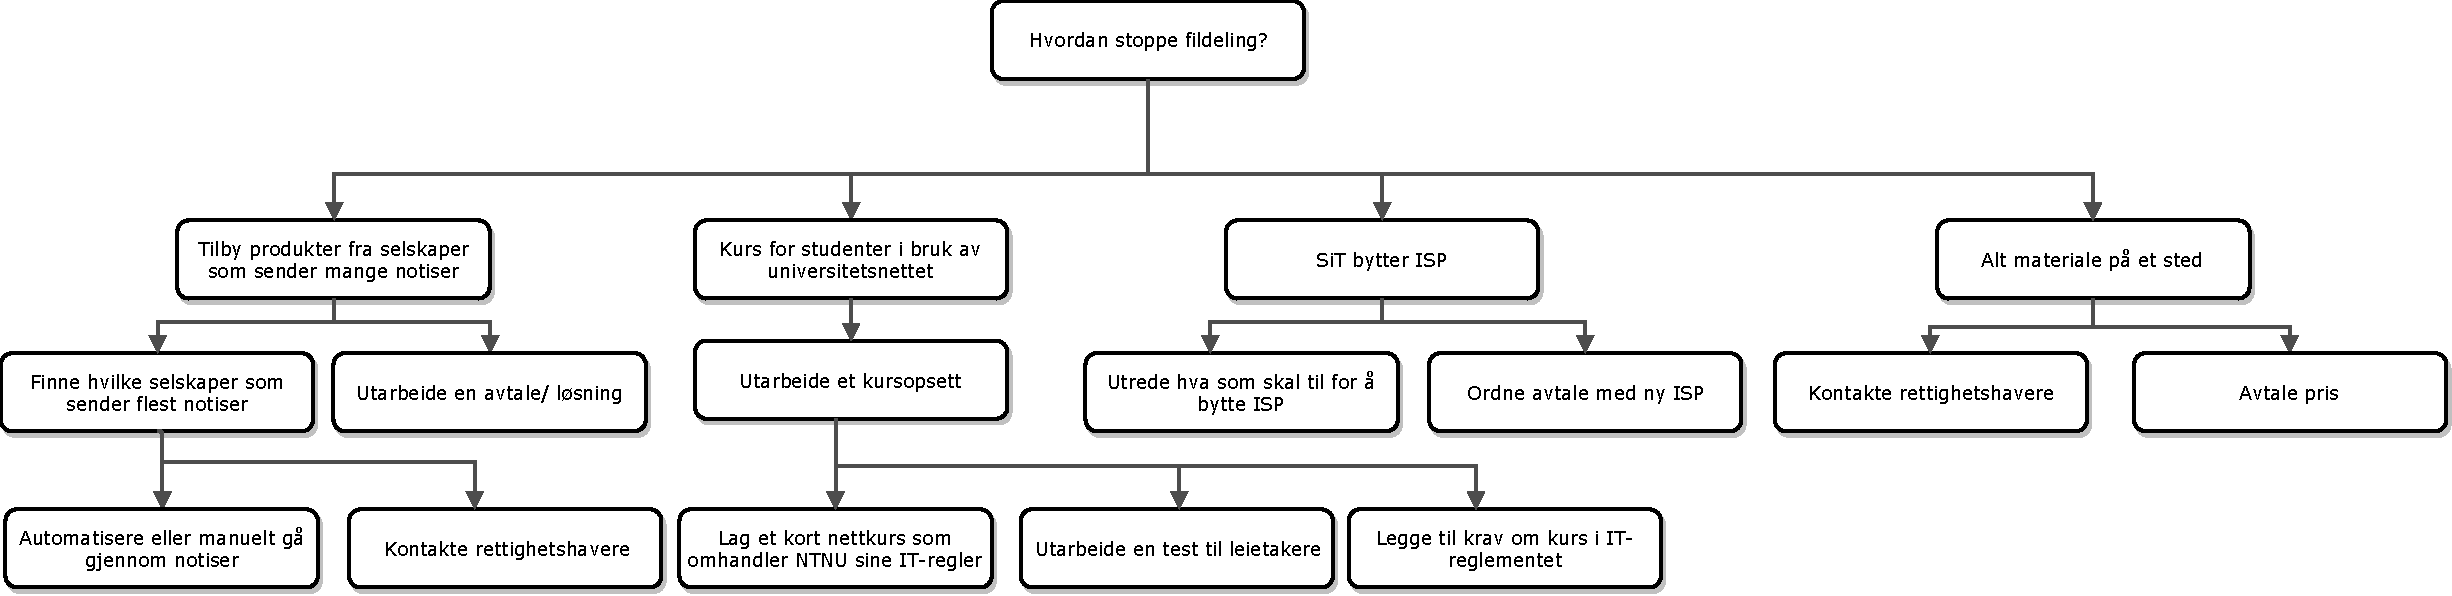
\includegraphics[scale=0.55, angle=90]{case_1/bilder/Tre-diagram.pdf}
    \caption[Trediagram til tiltak mot ulovlig fildeling]{Trediagram til tiltak mot ulovlig fildeling}
    \label{fig:case1-Tre-diagram}
\end{figure}

\section{Kostnad-nytte-analyse}
Denne seksjonen tar for seg en kostnad-nytte-analyse av nytteverdien til bruk av rotårsaksanalyse for case 1. 

\subsection{Kostnad for gjennomføring}
I denne analysen definerer vi kostnad som tid brukt på en iterasjonen av metoden. Vi definerer en skala for kostnad fra 1 til 5 der nivåene tilsvarer følgende tidsbruk:

\begin{enumerate}
    \item Under 50 timer
    \item 50-150 timer
    \item 150-250 timer
    \item 250-400 timer
    \item Over 400 timer
\end{enumerate}

Tabell \ref{tab:tidsbruk_case1} under viser tidsbruken i enkeltfasene i dette caset. Dette inkluderer tid brukt til å dokumentere alt som har med de enkelte fasene å gjøre. Dette er samlet tidsbruk fra fire personer. 

% Table generated by Excel2LaTeX from sheet 'Ark1'
\begin{table}[H]
  \centering
  \caption{Tidsbruk i de ulike fasene i case 1}
    \begin{tabular}{|lr|l|}
    \hline
    \multicolumn{3}{|c|}{\cellcolor{yellow}\textbf{Case 1}} \\ 
    \hline
    \multicolumn{1}{|l|}{\cellcolor{apricot}\textbf{Fase}} & \multicolumn{1}{l|}{\cellcolor{apricot}\textbf{Verktøy brukt}} & \cellcolor{apricot}\textbf{Timer totalt} \\
    \hline
    \multicolumn{1}{|l|}{Problemforståelse} & \multicolumn{1}{l|}{Flytdiagram og kritiske hendelser} & 16-20t \\
    \hline
    \multicolumn{1}{|l|}{Idémyldring} & \multicolumn{1}{l|}{Idémyldring} & 16-20t \\
    \hline
    \multicolumn{1}{|l|}{Datainnsamling} & \multicolumn{1}{l|}{Spørreundersøkelse} & 80-100t \\
    \hline
    \multicolumn{1}{|l|}{Datanalyse} & \multicolumn{1}{l|}{Analyseverktøy} & 100-120t \\
    \hline
    \multicolumn{1}{|l|}{Rotårsaksidentifisering} & \multicolumn{1}{l|}{Årsak-virkningsdiagram} & 14-18t \\
    \hline
    \multicolumn{1}{|l|}{Rotårsakseliminering} & \multicolumn{1}{l|}{6 tenkehatter og SIT} & 20-24t \\
    \hline
    \multicolumn{1}{|l|}{Løsningsimplementering} & \multicolumn{1}{l|}{Trediagram} & 14-20t \\
    \hline
    \multicolumn{2}{|l|}{\textbf{Sum}} & \textbf{260-322t} \\
    \hline
    \end{tabular}%
  \label{tab:tidsbruk_case1}%
\end{table}%

Dersom kosten på caset går over flere nivåer regner vi med medianen til ytterpunktene for å plassere kostnaden. Basert på kostnadsnivåene vi definerte over, plasseres tidsbruken på case 1 til:
\[Kostnad = 4\]

\subsection{Nytte av resultatene}
I denne analysen definerer vi nytten som egen oppfatning av hvor gode resultatene fra caset var. Det vurderes ut fra om vi tror det kan finnes andre underliggende årsaker, og hvorvidt vi mener problemet blir løst dersom rotårsakene fjernes, hvis det er gjennomførbart. Nytten defineres på en skala fra 1 til 5. 

I dette caset kom vi frem til at tilgjengeligheten på tjenester var i hovedsak rotårsaken til at studenter laster ned. Vi vurderer dette til å være relativt korrekt og at det ikke eksisterer så mange flere rotårsaker enn dette. Vi vurderte også økonomi og lav risiko som mindre rotårsaker. Eneste problemet med dette caset er at det er nærmest umulig for NTNU i seg selv å fjerne den første rotårsaken. Vi definerer derfor nytten til:
\[Nytte = 4\]

\subsection{Total nytteverdi}
Når vi regner ut kostnad-nytte deler vi kostnaden på nytteverdien. 
\[\frac{Kostnad}{Nytte} = Total nytteverdi\]

I dette caset blir regnestykket slik:
\[\frac{4}{4} = 1\]

Svarene på regnestykket kan bli fra 0,2 til 5. Jo lavere denne nytteverdien er, jo bedre fungerte metoden til caset. 